%--- Kapitel 11
\cleardoublepage
\chapter{Qualitätssicherung}
\label{sec:Kap-11}

Qualität und ihre Sicherung spielt bei allen technischen Produkten eine Rolle, doch ist der Name „Qualitäts\-sicherung“ für Laien in den meisten Fällen bereits eine Lüge. „Qualität“ ist nämlich nur ein relativer Begriff, und die Sicherung derselben kann auch bedeuten, dass ein Produkt stets in mittelprächtiger Qualität ausgeliefert wird, oder dass es nur in den meisten Fällen gewisse Qualitätsstandards erfüllt, Ausnahmen sind in einem geringen Umfang erlaubt.

\vspace{2mm} %%% für Druck

Bei Software ist es etwas anders, denn auch ein mehrfach verwendetes Softwareprodukt ist stets identisch, hat also dieselbe Qualität. Der Qualitätsanspruch an dieses Produkt hängt von den Anforderungen ab. Grundsätzlich sollte man erwarten können, dass wenigstens die funktionalen Anforderungen erfüllt werden. Bei den nichtfunktionalen Anforderungen muss man dagegen unterscheiden, ob die Erfüllung mess- oder beobachtbar ist. So kann man zum Beispiel auf die Verwendung einer bestimmten Plattform durchaus bestehen, aber Kriterien wie Wartbarkeit oder \mbox{Effizienz} sind kaum mit „erfüllt“ oder „unerfüllt“ bewertbar, wenn sie nicht genauer spezifiziert wurden.

\vspace{2mm} %%% für Druck

Konzentrieren wir uns also zunächst auf funktionale Anforderungen. Macht ein Software\-produkt das, was es soll? Wenn wir wieder in den technischen Bereich schauen, gibt es zur Beantwortung der Frage zwei Möglichkeiten: wir probieren es aus, oder aber wir entwickeln ein Produkt in einer Weise, dass es beweisbar die Anforderungen erfüllt. Bei einem Nussknacker mag das Ausprobieren mit großen Nüssen ausreichen, bei einer großen Eisenbahnbrücke sollte man eher davon absehen, die Brücke mit immer schwereren Zügen zu belasten, um zu sehen, ab wann sie zusammen\-bricht. Stattdessen gibt es statische Berechnungen, die schon bei der Konstruktion, Materialauswahl und -dimensionierung Eigenschaften der Brücke sicher\-stellen. 

\vspace{2mm} %%% für Druck

Bei der Softwareentwicklung ist es ähnlich: Ist ein Fehler der Software verschmerzbar und reparabel (und dies wird leider viel zu oft angenommen), so probiert man die Software an verschiedenen Beispielabläufen aus und nennt dies Test. Will man aber sicher sein, dass die Software korrekt ist, dann kann man dies unter Umständen auch beweisen. Wichtig ist, dass viel Testen fast nie einem Beweis gleichkommt, denn auch durch umfangreiche Tests kann nicht Korrektheit, sondern nur fehlende Korrektheit bewiesen werden. 

\vspace{2mm} %%% für Druck

Der bereits in Lektion~1 % TODO Lektion~\ref{sec:Lektion-1}
\marginline{Auf deutsch wird Dijkstra meist so zitiert:\\ \vspace{2mm} \textit{\small{„Durch Testen kann man nur die Anwesenheit von Fehlern feststellen, nicht aber ihre Abwesenheit.“}}}
erwähnte Edsger Dijkstra hat in seiner ACM Turing Lecture „The Humble Programmer“ 1972 den inzwischen berühmten Satz gesagt: 

\vspace{2.6mm} %%% für Druck

\sttpzitat{„Program testing can be a very effective way to show the presence of bugs, but it is hopelessly inadequate for showing their absence.“ \cite[864]{dij72}}{}

\vspace{2.6mm} %%% für Druck

Warum dies so ist, dazu später.

\vspace{0.4mm} %%% für Druck

Entsprechend ist dieses Kapitel grob in zwei Abschnitte aufgeteilt: Testen und Korrektheits\-beweise. Bevor wir einsteigen, eine kurze historische Einordnung. Seit etwa drei Jahrzehnten haben viele Informatiker die Vorstellung, dass zukünftig (immer relativ zu dem Zeitpunkt, als man die Vorstellung hatte) Softwareprodukte mathematische Objekte sein sollten, deren Korrektheit (bezogen auf gegebene Anforderungen) wie mathematische Theoreme bewiesen werden können. Mehr noch, per Konstruktion sollte die Korrektheit schon bei der Programmerstellung gegeben sein. Tatsächlich existieren Beweisverfahren für Programme schon sehr lange, wie Sie später lesen werden. Es gab und gibt dabei zwei Entwicklungsstränge:

Zum einen können Beweise für die Korrektheit eines Programms durch die Programmierer selbst oder durch andere Personen erstellt werden, so wie Menschen auch Beweise für mathematische Theoreme erstellen. Aber kann man einem der\-artigen Beweis trauen, oder enthält er – wie das Programm vielleicht auch – einen Fehler? Es gibt Ansätze, dass Beweise selbst durch entsprechende Werkzeuge geprüft werden. Diese Werkzeuge sind Programme, die die Korrektheit eines Beweises überprüfen können. Sie sind aber nicht in der Lage, selbst einen Beweis zu finden.

Der zweite Entwicklungsstrang geht einen Schritt weiter und betrachtet Programme, die bei Eingabe eines Softwareprodukts und seiner Spezifikation entscheiden, ob dieses Programm korrekt bezüglich der Spezifikation ist oder nicht. Diese sogenannten Model Checking Verfahren finden also selbst einen Beweis, sofern es einen Beweis gibt, und andernfalls ein Gegenbeispiel als Beweis für fehlende Korrektheit. Während noch vor einigen Jahrzehnten Model Checking nur auf recht kleine Software\-produkte anwendbar war, zeitigt es aufgrund der enorm gestiegenen Rechnerleistung und deutlich verbesserter Algorithmen heute auch bei größeren Programmen Erfolge.

Wir werden im zweiten Abschnitt nur kurz auf die erste Variante eingehen, also zeigen, wie man grundsätzlich die Korrektheit von Software beweisen kann, Model Checking dagegen weiterführenden Modulen überlassen.

Die Visionen der Wissenschaft Informatik führten dazu, dass man bis etwa vor 20~Jahren in der Informatikerausbildung Programmiersprachen vorgezogen hat, die sich für Korrektheitsbeweise besonders eignen -- wie gesagt in der Erwartung, dass einige Jahre später ein wildes drauf-los-Programmieren nur noch im Hobbybereich üblich sein würde, gerade so wie Architekten mit vernünftigen Plänen sich von Baumarktbastlern unterscheiden. Natürlich konnte man bereits damals sehen, dass der Schwachpunkt der Softwareentwicklung die Anforderungen sind, denn traditionelle Vorgehen basieren ja auf einigermaßen ausgereiften und stabilen Anforderungen, aber dieses Problem schien lösbar.

Wie ein Schock kam dann der Siegeszug der agilen Programmierung, der bereits im Kern den Vorstellungen der Wissenschaft widersprach, aber offensichtlich oft zu Softwareprodukten führte, die den Wünschen (um hier nicht Anforderungen zu sagen) der Kunden entsprachen, schneller zu entwickeln waren und auch nicht durch und durch fehlerhaft waren. Was sollte man nun mit dem Plan der Wissenschaft anfangen, wenn die Realität eine ganz andere Richtung ging? Für manch einen Informatik\-wissen\-schaftler sind agile Methoden immer noch Teufelszeug oder Bastelkram, andere haben sich auf die empirische Analyse der Wirksamkeit der Prinzipien agiler Methoden gestürzt und manche sind immer noch begeistert. Die meisten aber haben das agile Vorgehen achselzuckend zur Kenntnis genommen und bauen es, wie wir, in die Lehre ein, nach dem Motto: wenn schon, dann aber bitte richtig.

\vspace{1mm} %%% für Druck

Was hat der vorhergehende Abschnitt nun mit Qualitätssicherung zu tun? Während Tests in frühen Vorgehensmodellen zwar eine wichtige Rolle am Projektende spielten, sind sie bei agilem Vorgehen zentral. Man testet andauernd (programmiert also sehr im Stile von „Trial-and-Error“), spezifiziert mittels Testfällen und hat einen starken Glauben daran, dass genügend Tests eine stets ausreichende Qualitätssicherung darstellen. Dies ist in ganz vielen Fällen auch richtig, bei sogenannten sicherheits\-kritischen Systemen sollte man aber seine Ansprüche höher stellen, wie bei dem oben genannten Beispiel der Eisenbahnbrücke. Man denke auch an eine Robotersteuerung im medizinischen Bereich, an Software in der Luft- und Raumfahrt oder auch an den Einsatz von Softwarewerkzeugen an der Börse. Überall dort, wo Fehlfunktionen zu Katastrophen führen können, sollte man auch zukünftig die Qualität tatsächlich sicherstellen und auch beweisen.

\vspace{1mm} %%% für Druck

Neben Tests und Korrektheitsbeweisen gibt es weitere Konzepte, die mit der 
\linebreak %%% für Druck
Qualitäts\-sicherung von Software zu tun haben. Wir wollen an dieser Stelle vier Themenbereiche erwähnen:

\vspace{2mm} %%% für Druck

\minisec{Höhere Programmiersprachen}	

\vspace{0.5mm} %%% für Druck

Höhere Programmiersprachen nehmen dem Programmierer im Vergleich zu 
\linebreak %%% für Druck
maschinen\-nahen Sprachen vieles ab und bieten einen umfangreichen Befehlsvorrat an. Oft entspricht ein einzelner Befehl einer höheren Programmiersprache einem ganzen Programm einer anderen Sprache. Potentielle Fehler in diesem Programm werden also vermieden. Umgekehrt können der große Befehlsumfang und die vielfältigen Möglichkeiten Programmierer durchaus überfordern und so für eine zusätzliche Fehlerquelle sorgen. Aber es gibt auch andere Qualitätskriterien! So kann man besonders effiziente Programme, bezogen auf Speicherbedarf und Laufzeit, eher mit maschinennahen Sprachen herstellen.

\vspace{2mm} %%% für Druck

\minisec{Typisierung}	

\vspace{0.5mm} %%% für Druck

Verbunden mit dem vorigen Punkt ist die Typisierung von Programmiersprachen. Einerseits mag man es besonders komfortabel finden, wenn Variablen bzw. der ihnen zugeordnete Speicherplatz je nach Bedarf etwas Unterschiedliches repräsentieren, weil der jeweilige Datentyp nicht festgelegt ist. Viele Programmiersprachen nutzen gerade diese Variabilität aus, um vermeintlich besonders eleganten Code zu erlauben. Andererseits sind mit diesen vielen Möglichkeiten auch besonders viele Fehlermöglichkeiten verbunden, und ein strenger Umgang mit Datentypen hilft diese zu vermeiden.
	
\minisec{Wiederverwendung}	

Früher eine eher leere Floskel, heute gang und gäbe: einmal geschriebene Soft\-ware kann auf verschiedene Weise mehrfach verwendet werden. Sei es, dass sie in einer Programmbibliothek zur Verfügung gestellt wird und die Bibliothek bezüglich Qualitätsanspruch ein gewisses Vertrauen genießt. Oder sei es, dass man anstelle einer Neuprogrammierung zum Beispiel Open Source Programme übernimmt und entsprechend der Anforderungen modifiziert. Eine besondere, und auch besonders wenig kontrollierbare Form der Wiederverwendung ist durch ChatGPT gegeben; soll doch die KI die passende Vorlage finden und auch ihre Anpassung übernehmen. Dies gelingt überraschend oft überraschend gut.
	
\minisec{Code Inspection, Code Review, Statische Tests und Pair Programming}	
Diese vier Begriffe (die Übersetzung der englischen Begriffe in das Deutsche erscheint hier wenig sinnvoll) haben etwas gemein: Programmcode wird von Menschen be\-urteilt, ohne dass explizit Abläufe kreiert werden. Man mag darüber streiten, ob nicht jeder Mensch zum Verständnis eines Algorithmus oder eines Programms heimlich doch Ablauf"|fragmente im Kopf kreiert und betrachtet, aber dies geschieht hier jedenfalls nicht explizit. Natürlich erscheint dieses Vorgehen schwächer als systematische Tests oder Korrektheitsbeweise, doch ist auch die Perspektive des Programmierers zunächst rein statisch. Insofern können diese Verfahren doch bezüglich Qualitäts\-sicherung so gut sein wie sehr gute Programmierer.
	
Sie fanden die Behandlung dieser vier Themen zu oberflächlich und zu kurz? Zu Recht! Aber wir werden hier nicht mehr dazu erzählen, sondern in den Einsende\-aufgaben weitere Recherche und Gegenüberstellung Ihnen überlassen.


% 11.1
\clearpage
\section{Testen}
\label{sec:Kap-11-1}

Testen heißt zunächst einmal Ausprobieren, auch wenn im Software Engineering mit den Begriffen "`Test"' und "`testen"' viel mehr verbunden wird. Man testet ein beliebiges technisches Produkt, indem man ausprobiert, ob es das tut was es soll, funktionsfähig bleibt, andere Qualitätsanforderungen erfüllt usw. Umgekehrt ist nicht jedes Ausprobieren gleich ein Test: Man kann auch ein Produkt ausprobieren, um herauszufinden, was es tut oder um jemand anderem das Produkt zu demonstrieren. Beim Testen geht es dagegen grundsätzlich darum, Fehler zu finden oder Fehler\-freiheit wahrscheinlicher zu machen, wobei ein Fehler zunächst einmal ein Abweichen von der Vorstellung ist, wie das getestete System sich in einem bestimmten Fall verhalten sollte.

Beschränken wir uns auf Software. Wie bei dem Vergleich von Vorgehensmodellen in Lektion~1 % TODO Lektion~\ref{sec:Lektion-1}
diskutiert, betraf das Testen ursprünglich die fertige, implementierte Software, die erst relativ spät im Entwicklungsprozess vorliegt. Findet man hier einen Fehler, also ein anderes Verhalten als von der Spezifikation vorgegeben, hat man ein Problem: Liegt der Fehler an der Implementierung oder ist die Spezifikation fehlerhaft? Während ein Implementierungsfehler als Abweichung von der Spezifikation definiert werden kann, ist ein Spezifikationsfehler ein Abweichen von der Vorstellung der Stakeholder. Wie in Lektion~4 % TODO Lektion~\ref{sec:Lektion-4}
diskutiert, gleicht diese "`Vorstellung"' einem Wattebausch, der sich auch noch verändern kann. Aus diesem Grund werden Spezifikationen möglichst früh und immer wieder validiert, erste Prototypen mit den Anforderungen verglichen und in agilen Verfahren möglichst früh Software bereitgestellt, die von Beginn an Tests unterzogen wird, um den tatsächlichen Bedürfnissen der Stakeholder möglichst nahe zu kommen.
Wir wollen von den Überlegungen, wann und was im Rahmen verschiedener Prozesse bzw. Vorgehensmodelle getestet wird, in dieser Lektion weitgehend abstrahieren, und stattdessen Grundsätzliches zum Testen von Software herausstellen.

Es gibt zu Tests, Testverfahren, Testwerkzeugen, usw. etliche Bücher, die aber fast alle sehr praxisorientiert sind oder sich auf eine konkrete Programmiersprache beziehen. Insbesondere geht es vielfach um die Aufgaben und Qualifikationen zertifizierter Software-Tester, siehe zum Beispiel \cite{spi19}. Unsere Perspektive ist etwas anders, mit höherer Flughöhe und mehr an Standards und Prinzipien orientiert. An speziellen Test-Lehrbüchern haben wir uns nicht orientiert, sondern eher an Kapiteln zum Thema Test aus Büchern zum Softwareengineering. Als lesenswerte Beispiele empfehlen wir \cite{bal11}, \cite{lig09}, \cite{zel09} und \cite{lud23}. An vielen Stellen waren wir inspiriert von einem Vorlesungsskript von Martin Glinz \cite{gli05}.
\subsection{Wann wird getestet?}
\label{sec:Kap-11-1-1}

\minisec{Debugging}
Jeder Softwareentwickler 
\marginline{Debugging}
kennt es: Man schreibt ein Programmstückchen und probiert es gleich aus, schon um Tipp- oder Gedankenfehler zu entlarven. Dieses Vorgehen war in den Anfangszeiten der Computer weniger ausgeprägt, als die Eingabe stets über Lochkarten geschah und die Ausgabe eines Testlaufs erst Minuten oder Stunden später gedruckt vorlag – Bildschirme als Benutzungsschnittstelle gab es noch nicht. Damals hat man bereits aus Effizienzgründen sehr genau hingeschaut, ob das Programmstückchen syntaktisch korrekt ist und wohl das Gewünschte leistet. Heutzutage sind kleine Testläufe in Sekunden erledigt, und entsprechend haben sich Programmierer daran gewöhnt, diese auch regelmäßig durchzuführen. Es geht dabei darum zu prüfen, ob das Programm überhaupt läuft und ob es das leistet, was der Programmierer gerade implementieren wollte, häufig abgeleitet aus der Spezifikation des Programms. Läuft das Programm nicht oder sind die Ergebnisse offensichtlich falsch, wird das Programm verbessert und wieder getestet.

Man nennt dieses Vorgehen auch \emph{Debugging}\footnote{von \emph{Bug}, was eigentlich Käfer heißt, aber in der Computersprache Fehler bezeichnet; im Internet finden sich viele nette Geschichten, wie es zu diesem Namen für Fehler kam.}. Wenn das Programm läuft und die Ergebnisse den Vorstellungen des Entwicklers entsprechen, wird das Debugging beendet.

Wichtig ist, dass beim Debugging Missverständnisse bei der Interpretation der Spezifikation nicht erkannt werden, denn der Programmierer hat ja beim Schreiben und beim Testen des Programms dieselbe, vielleicht falsche, Vorstellung. Auch kann es sein, dass der Programmierer zwar die Spezifikation richtig verstanden hat, aber bei der Implementierung gewisse Sonderfälle schlicht übersehen hat. Auf diese wird er dann natürlich beim Debugging auch nicht kommen.

Debugging beschränkt sich nicht auf eine Analyse des Eingabe- / Ausgabeverhaltens, also auf die Frage, ob ein Programm das leistet, was in der Spezifikation versprochen wurde. Insbesondere dann, wenn dies nicht der Fall ist, will man mehr über das tatsächliche Verhalten des Programms wissen. Grob gesagt, hat der Entwickler eine Vorstellung davon, wie das Programm für bestimmte Eingaben abläuft und zum Ergebnis kommt. Nun will er wissen, ob der Programmablauf tatsächlich dieser Vorstellung entspricht. Oder, falls das Ergebnis fehlerhaft ist, an welcher Stelle es erste Abweichungen gab.

Eine recht alte Möglichkeit, den Programmablauf zu "`überwachen"', ist die Ausgabe von Variablenwerten an verschiedenen Stellen des Programms. Bei geschickter Wahl der überwachten Variablen und Programmstellen für die Ausgabe erhält man so ein hinreichendes Bild von einem Ablauf. Allerdings kann die Ausgabe recht umfangreich sein. Zudem ist es oft sehr arbeitsaufwändig, alle Werte nachzuvollziehen und zu kontrollieren. Ein weiterer Nachteil ist, dass diese Ausgabebefehle während des Debuggings immer wieder hinzugefügt und entfernt werden müssen -- und schließlich ganz gestrichen werden.

Eine Alternative, die von manchen Programmiersprachen angeboten wird, greift auf das Konzept der Zusicherungen (assertions)
\marginline{Zusicherungen}
zurück, das wir in Abschnitt~9.2.1 % todo Abschnitt~\ref{sec:Kap-9.2.1}
bereits eingeführt haben. Eine Zusicherung ist ein logischer Ausdruck, der meist den Wert einer Variablen durch Kombination anderer Variablenwerte beschreibt, aber auch andere Zusammenhänge zwischen Variablenwerten sind möglich. Zusicherungen werden in den Programmcode an relevante Stellen geschrieben. Mit der Zusicherung wird ausgedrückt, welchen Variablenwert man an dieser Stelle erwartet. Eine Zusicherung sollte erfüllt sein, nachdem die davor stehende Anweisung ausgeführt wurde, andernfalls liegt ein Fehler vor und eine entsprechende Fehlermeldung wird ausgegeben. "`Fehler"' bedeutet hier, dass der Programmierer einen Fehler gemacht hat und das Programm nicht so läuft, wie er es sich vorgestellt hat. Entsprechende Fehlermeldungen sind deshalb sehr hilfreich, um entsprechende Gedankenfehler bei der Programmierung zu entdecken. Nach der Testphase kann die Überprüfung der Zusicherungen global ausgeschaltet werden, so dass im Betrieb keine Laufzeit\-beeinflussung vorliegt.

Zusicherungen und durch sie ausgelöste Fehler sind unbedingt zu unterscheiden von Ausnahmen (exceptions). Diese beschreiben nicht Programmfehler, sondern Datenfehler bzw. Abweichungen von erwarteten Dateneigenschaften. Während im korrekten Programm Zusicherungen immer erfüllt sind, können Ausnahmen immer vorkommen. Deshalb werden Zusicherungen beim Einsatz eines Softwareprodukts nicht mehr überprüft, Ausnahmen aber sehr wohl.

\minisec{Unsystematisches Testen}
Der jetzt 
\marginline{Wegwerf-Test}
beschriebene Einsatz von Testverfahren hat keinen wirklichen Namen und wird manchmal als "`Wegwerf-Test"' bezeichnet. Er liegt irgendwo zwischen Debugging und dem systematischen Test. Der Ersteller einer Software selbst oder jemand anders führt das Programm für irgendwelche Eingabedaten aus. Findet man dabei Fehler, so wird entweder das Problem an den Programmierer zurückverwiesen, oder aber es wird der Grund für den Fehler gleich gesucht, um das Programm zu korrigieren. Dabei könnten allerdings neue Fehler entstehen, doch das wird beim unsystematischen Testen durch entsprechende Vorsicht und Einsicht in das Programm und seine Funktionsweise versucht zu vermeiden. Man testet so lange bis man meint, dass es genug sei und die Überzeugung erlangt, dass das Programm grundsätzlich für alle gültigen Eingaben läuft und leistet was es soll.

Da die Testläufe weder geplant noch dokumentiert werden, ist es sehr gut möglich, dass dieselben Tests wiederholt durchgeführt werden, ohne dass dies zu neuen Erkenntnissen führt (deshalb "`Wegwerf-Test"'). Insbesondere wenn das Testen vom Programmierer selbst durchgeführt wird, bestehen ansonsten dieselben Nachteile wie beim Debugging.

Meist kann die tatsächliche Ausgabe einer Programmausführung nicht sogleich geprüft werden, da die entsprechende korrekte, zu erwartende Ausgabe erst ermittelt werden muss. Auch hierin liegt eine Fehlerquelle, weil manchmal die Programm\-ausgabe fälschlich als korrekt vermutet wird und ihr mehr Vertrauen geschenkt wird als der aus anderen Gründen oft fehlerhaften händisch\footnote{"`händisch"' heißt hier natürlich nicht wirklich mit den Händen, sondern nur ohne Rechner\-unterstützung; manchmal sagt man auch "`zu Fuß"'.} ermittelten vermeintlichen Soll-Ausgabe. 

\minisec{Systematisches Testen}
\begin{itemize}
	\item Der erste wichtige 
	\marginline{Test-Spezialisten}
	Unterschied zu den bisher genannten Tests ist, dass nun die Tests von \emph{Spezialisten für das Testen} durchgeführt werden, insbesondere also nicht vom Programmierer der Software bzw. nicht allein von ihm. Die Tests sind geplant. Eingaben und entsprechende Ausgaben, die das Programm liefern soll, existieren bereits, bevor das Programm ausgeführt wird. Diese werden \emph{Testfälle} genannt.

	\item Für das Testen 
	\marginline{Testvorschrift}
	selbst, also für die Erstellung der Testläufe, liegt eine \emph{Test\-vorschrift} vor, die auch weitere Bedingungen für Testläufe beschreibt und dadurch die Ergebnisse reproduzierbar macht. 

	\item Soll-Resultate 
	\marginline{Soll-Resultate}
	liegen vor Durchführung der Tests vor und können sofort mit den Ist-Resultaten verglichen werden. 

	\item Es geht nicht 
	\marginline{Analyse}
	sofort darum, Ursachen für Fehler zu finden und die Fehler zu bereinigen, sondern zunächst um eine umfassende Analyse des Verhaltens einer nicht andauernd geänderten Programmversion.

	\item Die Testergebnisse
	\marginline{Dokumentation}
	werden dokumentiert.
\end{itemize}

Natürlich werden als fehlerhaft erkannte Programme nach einem systematischen Test auch korrigiert; Fehler können aus den nicht bestandenen Testläufen ermittelt werden. Anschließend wird der Test wiederholt, wobei meist alle Testfälle wiederholt werden. Dafür werden oft automatisierte Tests eingesetzt, um den manuellen Aufwand klein zu halten. Wenn zuvor genannte \emph{Testziele}
\marginline{Testziele}
erreicht wurden, endet das Verfahren.
\subsection{Was wird getestet?}
\label{sec:Kap-11-1-2}

Ein großes Softwaresystem setzt sich aus Komponenten zusammen. Aus der Gesamt\-spe\-zi\-fi\-ka\-tion muss eine Spezifikation für diese Komponenten folgen, so dass aus der Korrektheit der Komponenten bezüglich dieser Spezifikationen und dem Zusammenspiel der Komponenten die Korrektheit des Gesamtsystems folgt. Grob unterscheidet man die Zerlegung eines Systems in Teilsysteme, die wiederum aus Modulen bestehen. Entsprechend gibt es folgende Unterscheidung (s.~Abb.~\ref{fig:puzzle_testen}):

% Abbildung händisch verschoben.
% Hier gehört die Abbildung {fig:puzzle_testen} eigentlich hin.

\begin{itemize}
	\item \textit{Komponententest} bzw. \textit{Modultest} (engl. unit test), 
	\marginline{Komponenten\-test}
	hier werden die einzelnen Komponenten bzw. Module getestet.
	\item \textit{Integrationstest} (engl. integration test), 
	\marginline{Integrationstest}
	hier wird das Zusammenspiel der 
	\linebreak %%% für Druck
	Module auf Teilsystemebene getestet.
	\item \textit{Systemtest} (engl. system test)
	\marginline{Systemtest}
\end{itemize}

Bis hierhin geht es beim Testen stets darum, Fehler zu finden. Tatsächlich ist dies der besondere Ehrgeiz der Tester, und sie sind entsprechend in den Qualitäts\-verbesserungs\-prozess eingebunden. Fast kann man sagen: Wer keine Fehler findet, hat seinen Job schlecht gemacht. Irgendwann aber muss der Prozess beendet sein und das System ausgeliefert werden. Zu diesem Zeitpunkt führt man nochmal einen Test durch:

\begin{itemize}
	\item \textit{Abnahmetest} (engl. acceptance test), 
	\marginline{Abnahmetest}
	hier sollten keine Fehler mehr gefunden bzw. aufgedeckt werden, so die Hoffnung.
\end{itemize}

\begin{figure}[h!]
	\centering
	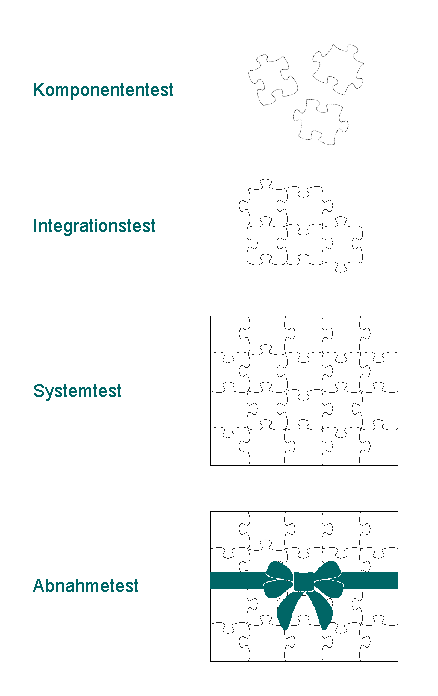
\includegraphics[width=0.55\textwidth]{Bilder/Kapitel-11/Puzzle_Testen.pdf}
	\caption[Illustration Teststrategien]{Illustration angelehnt an \cite{gli05}}
	\label{fig:puzzle_testen}
\end{figure}
\subsection{Wie wird getestet?}
\label{sec:Kap-11-1-3}

Ein \textit{Testablauf} 
\marginline{Testablauf}
ist nicht etwa der Ablauf des Programms für einen Testfall, sondern soll hier den gesamten Prozess des \textbf{systematischen Testens} eines Software\-produkts skizzieren.

\minisec{Planung}

Naturgemäß geht es mit der Planung der Tests los. Dazu gehört die \textit{Teststrategie}: 
\marginline{Teststrategie}
Welche Programmfragmente sollen zu welchem Zeitraum bzw. in welcher Phase getestet werden, wie soll dies geschehen (automatisch oder manuell, und durch wen), und wie viel Zeit steht dafür zur Verfügung? Ein ausgewähltes Programmfragment wird im Folgenden „Prüfling“ genannt.
	
\minisec{Vorbereitung}

Im Unterschied zu niederschwelligen Tests 
\marginline{Test\-vorbereitung}
sollen systematische Tests klar definiert und reproduzierbar sein. Deshalb sind bei der Vorbereitung der Tests die Auswahl der Testfälle festzulegen und die Testumgebung wird bereitgestellt. Zudem geht es hier um die präzise Angabe der Testvorschrift, die auch die Umgebung und Rahmen\-bedingungen mit einschließt.
	
\minisec{Durchführung}

Die in der Vorbereitung bereitgestellte Testumgebung wird eingerichtet 
\marginline{Test\-durchführung}
und die Testfälle werden gemäß Testvorschrift ausgeführt (genau genommen ist nur dieser Schritt das eigentliche Testen). Jeder Testfall enthält eine Eingabe und die gemäß Spezifikation dazugehörige Ausgabe, auch Soll-Ausgabe genannt. Die tatsächlichen Ausgaben werden mit der Soll-Ausgabe verglichen und dokumentiert. Auch bzw. erst recht falsche Ausgaben sind eine für die Verbesserung des Programms wertvolle Information. Wie bereits erwähnt, wird der Prüfling während der Testdurchführung nicht verändert, auch wenn Fehler bereits offenbar wurden.
	
\minisec{Auswertung}

Erst nach der vollständigen Durchführung des Tests 
\marginline{Testauswertung}
für alle vorgesehenen Testfälle findet eine Auswertung des Tests statt. Die Testbefunde, also eventuelle Abweichungen der tatsächlichen Ausgaben von den Soll-Ausgaben werden zusammengestellt und dokumentiert. Im Rahmen der Auswertung wird auch festgestellt, ob der Test als erfolgreich angesehen wird oder nicht. Erfolg bedeutet nicht in jedem Fall 100\,\% korrekte Ausgaben, sondern auch geringere Werte sind grundsätzlich als Erfolgs\-kriterium denkbar. Insbesondere können Testfälle, die sich nicht direkt auf den vorgesehenen Eingabebereich beziehen, positiv oder negativ ausfallen. Dies hat nichts mit der eigentlichen Spezifikation zu tun. Ein Programm, das außerhalb seines definierten Eingabebereichs sinnvolle Ausgaben ausgibt, wird \textit{robust} genannt, und Robustheit 
\marginline{Robustheit}
ist auch ein Qualitätskriterium. Je nach Anwendungsbereich wird gefordert, dass eine ungültige Eingabe als solche identifiziert und abgewiesen wird, oder dass -- sofern möglich -- eine zur Spezifikation analoge Funktionalität erfüllt wird. Ein Beispiel für den ersten Fall ist die Division durch 0. Hier gibt es kein vernünftiges Ergebnis und insbesondere ist gar kein Ergebnis (zum Beispiel durch eine Endlosschleife oder durch einen Programmabsturz) keine robuste Erweiterung der Programmfunktionalität. Ein Beispiel für den zweiten Fall ist die Addition von ganzen Zahlen, auch wenn nur die Addition positiver ganzer Zahlen spezifiziert wurde. 

\vspace{\baselineskip}

Nicht zum Test selbst gehört die

\minisec{Fehlerbehebung,}

die auf der Analyse der gefundenen Abweichungen zwischen tatsächlichem Verhalten und Soll-Verhalten basiert. Ziel der Analyse ist die Bestimmung der Fehlerursachen. In vielen Fällen kann man diese dann einfach beheben. Manchmal entstehen dabei allerdings unerwartete neue Fehler -- deswegen muss in der nächsten Runde der gesamte Test wiederholt werden. Es ist auch denkbar, dass der gefundene Fehler nicht leicht zu reparieren ist. So ist zum Beispiel bei Auswahl des falschen Algorithmus für eine algorithmische Aufgabenstellung keine lokale Änderung fehlerbehebend, sondern eine andere Auswahl des gesamten Algorithmus. Es ist dann also ein neues Programm zu schreiben.

\subsection{Funktionsorientierter Test (Black-Box-Test)}
\label{sec:Kap-11-1-4}

Die Testfälle beim funktionsorientiertem Test werden ausschließlich aufgrund der Spezifikation erstellt. 
Black-Box heißt, dass der Programmcode selbst dem Tester nicht bekannt ist bzw. bekannt sein muss. Er spielt bei der Bestimmung der Testfälle jedenfalls keine Rolle.

Mögliche Ziele beim funktionsorientiertem Test sind:
\begin{itemize}
	\item Funktionsüberdeckung: jede spezifizierte Funktion wird einmal aktiviert,
	\item Ausgabeüberdeckung: jede Ausgabe wird wenigstens einmal erzeugt, 
	\item Ausnahmeüberdeckung: jede Ausnahme wird wenigstens einmal erzeugt.
\end{itemize}

Neben Einhaltung der funktionalen Anforderungen kann es auch um spezifizierte Leistungsanforderungen gehen, gerade auch unter ungünstigen Bedingungen
\linebreak %%% für Druck
(Belastungs\-tests).

Wie sollen die Testfälle ausgewählt werden? Natürlich könnte man zunächst vermuten: je mehr desto besser. Dies ist aber nicht die ganze Wahrheit, denn sehr viele Testfälle bedeuten auch sehr viel Testaufwand, der im Zweifel zu kostenaufwändig und insbesondere zu zeitaufwändig ist. Vielmehr ist es wichtig, dass die Testfälle ausgewählt werden, die mit einer gewissen Wahrscheinlichkeit Fehler aufdecken. Wenn Testfälle sich wahrscheinlich gleichen (deckt einer einen Fehler auf, dann der andere auch, und umgekehrt), so reicht die Betrachtung einer dieser Testfälle. Grob gesagt gilt für die Auswahl: Soviel wie nötig (existierende Fehler sollen gefunden werden) und dabei so wenig wie möglich (Effizienz).

Wir wollen als Beispiel den Algorithmus zur Berechnung des größten gemeinsamen Teilers (ggT) zweier natürlicher Zahlen aus Lektion~1 % TODO Lektion~\ref{sec:Lektion-1}
wieder aufgreifen. Abbildung~\ref{fig:flussdiagramm_in_Kap-11} zeigt das Flussdiagramm nochmal.

\begin{figure}[h!]
	\centering
	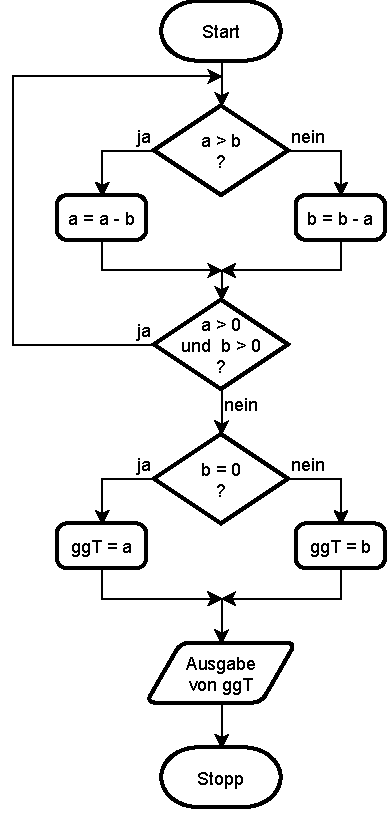
\includegraphics[scale=0.75]{Bilder/Kapitel-1/Abb-1-4.pdf}
	\caption[Der Euklidische Algorithmus als Flussdiagramm]{Ein Flussdiagramm, das den Euklidischen Algorithmus zur Be\-rechnung des größten gemeinsamen Teilers (ggT) zweier positiver Ganzzahlen grafisch darstellt}
	\label{fig:flussdiagramm_in_Kap-11}
\end{figure}


\minisec{Äquivalenzklassen}

Wenn man vermuten kann, dass ein Programm für zwei unterschiedliche Eingaben entweder in beiden Fällen korrekt läuft oder in beiden Fällen einen Fehler aufweist, so reicht es, eine der beiden Eingaben zu testen.

\vspace{1mm} %%% für Druck

Beispiel ggT-Algorithmus aus Abbildung~\ref{fig:flussdiagramm_in_Kap-11}: % TODO Kapitel~\ref{sec:Kap-2.1}:

\vspace{1mm} %%% für Druck

mögliche Äquivalenzklassen:

\begin{addmargin}[25pt]{25pt}
	$a>b>1$, \dasHeisst alle Werte von $a$ und $b$, für die $a>b>1$ gilt.
	
	$b>a>1$
	
	$a=b>1$
	
	$a=1$
	
	$b=1$
	
	$a=b=1$
\end{addmargin}

Man nennt diese Eingaben dann äquivalent und betrachtet entsprechende Äqui\-valenz\-klassen von Testfällen (streng genommen sind es keine Äquivalenzklassen, denn sie sind nicht notwendigerweise disjunkt).

\vspace{2mm} %%% für Druck

\minisec{Grenzwertanalyse}

An den Grenzwerten treten häufig Fehler auf. Die Grenzwerte können sowohl technischer Natur sein, also zum Beispiel die Darstellbarkeit der betroffenen Zahlen berühren. Oder aber sie sind durch den implementierten Algorithmus begründet.

\vspace{1mm} %%% für Druck

Beispiel ggT-Algorithmus:

\begin{addmargin}[25pt]{25pt}
	$a, b$ sehr groß
	
	$a,b$ sehr klein
\end{addmargin}

Die Grenzwertanalyse ist insbesondere relevant bei reellwertigen Eingaben.

\vspace{2mm} %%% für Druck

\minisec{Ursache-Wirkungsgraph}

Das ist bei Black-Box-Verfahren weniger einfach, weil die Programmstruktur nicht mit einbezogen werden darf. Es geht darum Eingaben zu finden, die bestimmte Ausgaben und insbesondere besondere Reaktionen wie Ausnahmen erzeugen.

\vspace{1mm} %%% für Druck

Beispiel ggT-Algorithmus:

\begin{addmargin}[25pt]{25pt}
	$a,b$ teilerfrei
	
	$a$ Vielfaches von $b$
	
	$b$ Vielfaches von $a$
\end{addmargin}

\vspace{2mm} %%% für Druck

\minisec{Ungültige Eingaben}

Beispiel ggT-Algorithmus:

\begin{addmargin}[25pt]{25pt}
	$a= 0$
	
	$b<0$
\end{addmargin}

\pagebreak %%% für Druck
\subsection{Strukturorientierter Test (White-Box-Test)}
\label{sec:Kap-11-1-5}

Der Name White-Box ist eigentlich nicht korrekt, denn in eine weiße Kiste kann man so wenig hineinschauen wie in eine schwarze. Deshalb wird manchmal auch Glass-Box-Test gesagt. Bei dieser Variante ist die, also nun sichtbare, Programmstruktur zusätzliche Grundlage bei der Auswahl der Testfälle. Natürlich geht die Spezifikation ebenfalls ein, denn sie bestimmt ja die gewünschten Ausgaben.

\vspace{2mm} %%% für Druck

Wir betrachten wieder den ggT-Algorithmus aus Abbildung~\ref{fig:flussdiagramm_in_Kap-11}. Da wir ja beim strukturorientiertem Test die Programmstruktur verwenden dürfen, wollen wir sie explizit angeben (Algorithmus~\ref{algo:berechnung_ggt}). Eigentlich ist es eine unmittelbare Übersetzung aus dem Flussdiagramm. Statt einer konkreten Programmiersprache verwenden wir eine übliche Notation im sogenannten Pseudo-Code.

\vspace{\baselineskip} %%% für Druck
\vspace{\baselineskip} %%% für Druck

\begin{algorithm}[H]
	\caption{Algorithmus zur Berechnung des ggT}
	\label{algo:berechnung_ggt}
	
	\vspace{2mm} %%% für Druck
	\vspace{\baselineskip}
	
	\KwData{Eingabe: $a,b \geq 1$}
	\KwResult{Ausgabe: $\ggt (a,b)$}
	
	\vspace{2mm} %%% für Druck
	\vspace{\baselineskip}
	
	\Repeat{$a=0 \vee b=0$}{
		\eIf{$a > b$}{
			$a = a - b$
		}{
			$b = b - a$
		}
	}
	
	\vspace{2mm} %%% für Druck
	\vspace{\baselineskip}
	
	\eIf{$a=0$}{
		\Return{$b$}
	}{
		\Return{$a$}
	}
	
	\vspace{2mm} %%% für Druck
	\vspace{\baselineskip}
\end{algorithm}

\vspace{\baselineskip} %%% für Druck
\vspace{\baselineskip} %%% für Druck

\minisec{Anweisungsüberdeckung} % ist absichtlich nur noch \minisec

\vspace{2mm} %%% für Druck

\textit{Anweisungsüberdeckung} 
\marginline{Anweisungs\-überdeckung}
bedeutet, dass jede Anweisung des Programms wenigstens in einem Testfall ausgeführt wird. So kann man einerseits erkennen, ob ein Befehl grundsätzlich fehlerhaft ist. Hätten wir im ggT-Algorithmus zum Beispiel statt der Anweisung $a=a-b$ die Anweisung $a=a-b-1$ verwendet, so liefert das so modifizierte Programm immer einen falschen Wert, wenn jemals zu Schleifenbeginn $a>b$ gilt, die falsche Anweisung also auch ausgeführt wird. Deshalb muss für eine Anweisungsüberdeckung sichergestellt werden, dass dies auch für wenigstens einen Testlauf der Fall ist.

\pagebreak %%% für Druck

In diesem Beispiel ist das besonders einfach, wir können zum Beispiel die Anfangswerte $a=3$ und $b=2$ verwenden. Dann gilt beim ersten Schleifendurchlauf $a>b$, und die Ausführung der fehlerhaften Anweisung $a=a-b-1$ ergibt den Wert 0 für $a$. Die Schleife wird verlassen, weil $a=0 \vee b= 0$ zu \emph{wahr} ausgewertet wird (die erste Teilbedingung ist \emph{wahr}, $\vee$ ist das logische \emph{oder}, und damit ist der gesamte Ausdruck \emph{wahr}). Anschließend ist bei der \textbf{if}-Abfrage $a=0$ erfüllt, und es wird der Wert von $b$ ausgegeben. Dieser ist weiterhin 2, aber 2 ist nicht der größte gemeinsame Teiler von 2 und 3.

\vspace{2.75mm} %%% für Druck

Für die Anweisungsüberdeckung reicht dieser eine Testlauf allerdings nicht aus, denn weder die Anweisung $b=b-a$ wurde ausgeführt, noch die Anweisung \textbf{return} $a$. Beginnen wir deshalb auch mit den Werten $a=2$ und $b=2$. Dann gilt $a>b$ nicht und es wird $b=b-a$ ausgeführt. Als Ergebnis erhalten wir den Wert 0 für $b$. Die Schleife wird wiederum verlassen, und nun wird der in diesem Fall korrekte Wert 2 (der Wert von $a$) ausgegeben. In beiden Testläufen zusammen wurden alle Anweisungen jeweils mindestens einmal ausgeführt, die Anweisungsüberdeckung ist damit gegeben.

\vspace{2.75mm} %%% für Druck

In diesem Trivialbeispiel reichte es aus, die Verzweigungen mit entsprechenden Eingaben zu "`steuern"'. Dies ist natürlich nicht immer so einfach, weil die für die Verzweigungsbedingungen relevanten Variablenwerte sich durch andere Zuweisungen in unübersichtlicher Weise ergeben könnten. So wie man Fehler beim Programmieren machen kann, ist dies auch beim Testen möglich. Man muss deshalb genau prüfen, dass alle Anweisungen tatsächlich ausgeführt werden.

\vspace{2.75mm} %%% für Druck

Es ist übrigens nicht immer notwendig, für alle Zweige einer Verzweigung jeweils eigene Testläufe zu kreieren. Beginnen wir mit $b=3$ und $a=2$, so gilt beim ersten Schleifendurchlauf $a>b$ nicht, beim zweiten Schleifendurchlauf dagegen (nachdem $b$ mit 1 überschrieben wurde) gilt $a>b$. Mit einer Ausführung lassen sich hier also beide Zweige überdecken.

\vspace{2.75mm} %%% für Druck

Kehren wir zurück zum Algorithmus, wie er im Flussdiagramm und als Algorithmus~\ref{algo:berechnung_ggt} beschrieben ist (also mit der Anweisung $a=a-b$ statt $a= a-b-1$). Wir wollen auch für diesen (offenbar korrekten) Algorithmus Testläufe erstellen, die alle Anweisungen überdecken. Versuchen Sie es doch einmal! Ihnen wird auffallen, dass die Bedingung $a=0$ nach der Schleife nie erfüllt ist und Sie somit die Anweisungsüberdeckung nicht erreichen, obwohl das Programm für alle gültigen Eingaben das korrekte Ergebnis liefert. Das Programm ist daher im formalen Sinne korrekt, aber die Anweisungsüberdeckung ist nicht möglich.

\vspace{2.75mm} %%% für Druck

Wie kommt das? Zu Beginn gilt $a>0$. Um nach der Schleife $a=0$ zu erfüllen, müsste $a$ in der Schleife auf 0 gesetzt werden. Nur die Anweisung $a=a-b$ schreibt einen neuen Wert für $a$. Der Ausdruck $a-b$ kann aber an dieser Stelle niemals 0 sein, denn die Anweisung wird nur ausgeführt, wenn $a>b$ gilt.

\vspace{2.75mm} %%% für Druck

Auch wenn das Programm also korrekt ist, gelingt die Anweisungsüberdeckung nicht, und dies ist immerhin ein Zeichen dafür, dass der Programmierer nicht genau verstanden hat, was er da schreibt. 

\pagebreak %%% für Druck

Versuchen wir (eine zugegebenermaßen einfältige) Reparatur:

\vspace{2mm} %%% für Druck

\begin{algorithm}[H]
	\caption{Erster Reparaturversuch}
	\label{algo:erster_reparaturversuch}

	\vspace{\baselineskip}

	\KwData{Eingabe: $a,b \geq 1$}
	\KwResult{Ausgabe: $\ggt (a,b)$}

	\vspace{\baselineskip}

	\Repeat{$a=1 \vee b=1$}{
		\eIf{$a > b$}{
			$a = a - b$
		}{
			$b = b - a$
		}
	}

	\vspace{\baselineskip}

	\eIf{$a=1$}{
		\Return{$a$}
	}{
		\Return{$b$}
	}
	
	\vspace{\baselineskip}
\end{algorithm}

\vspace{\baselineskip} %%% für Druck

Statt $a=0 \vee b=0$ lautet die Schleifenabbruchbedingung nun $a=1 \vee b=1$. Falls $a=1$ wird $a$ ausgegeben, falls $b=1$ wird $b$ ausgegeben. Die falsche Überlegung ist, dass die Differenz gar nicht 0 werden muss; bei zwei Zahlen mit einer Differenz von 1 ist doch klar, dass der größte gemeinsame Teiler 1 lautet, und die fortgesetzte Subtraktion der 1 von der anderen Zahl erscheint unnötig. Wenn man genauer schaut, sieht man, dass das Ergebnis einer Ausführung nur 1 lauten kann! Entsprechend hätte man nach der Schleife auch gleich den Wert 1 ausgeben können.

\vspace{2mm} %%% für Druck

Nun führen wir zwei Testläufe zur Anweisungsüberdeckung durch, zum Beispiel für die Zahlenpaare $a=4$, $b= 5$ und dann für $a=5$, $b=4$. In beiden Fällen kommt das richtige Ergebnis heraus und alle Anweisungen wurden wenigstens einmal durchgeführt. Dies sollte allerdings nicht überraschen, denn Anweisungsüberdeckung ist, wie alle Testkriterien, keine hinreichende Bedingung für Korrektheit.
\vspace{2mm} %%% für Druck

\minisec{Zweigüberdeckung} % ist absichtlich nur noch \minisec

\vspace{2mm} %%% für Druck

So ganz falsch war unsere Überlegung bei dem zuletzt betrachteten, fehlerhaften Algorithmus (Algorithmus~\ref{algo:erster_reparaturversuch}) aber doch nicht: Wird die Schleife nur einmal ausgeführt, dann ist das Ergebnis immer richtig! Erst wenn die Schleife mindestens ein zweites Mal ausgeführt wird, kann etwas Unerwünschtes passieren. Wann immer im Pro\-gramm\-ab\-lauf zu Beginn der Schleife $a=b>1$ gilt, gilt am Ende der Schleife $a>0 $ und $b=0$. Die Schleife wird also nicht verlassen, aber auch ihre nächste Ausführung ändert die Werte von $a$ und $ b $ nicht mehr. Also wird die Schleife wieder und wieder ausgeführt und die Abbruchbedingung nie erfüllt. Nun ist "`gar kein Ergebnis"' natürlich fast so schlimm wie ein falsches Ergebnis. Dieser Testlauf zeigt also, dass das Programm nicht korrekt ist. Um ihn allerdings zu finden, reichte die Anweisungsüberdeckung nicht aus. Erst wenn die Schleifenabbruchbedingung einmal zu \emph{falsch} ausgewertet wird, kann man den Fehler sehen. Eine reine Anweisungs\-über\-deckung fordert aber nicht, dass jede Bedingung, sei sie im Kontext einer Verzweigung oder einer Schleife, mit beiden möglichen Auswertungen \emph{wahr} und \emph{falsch} in den Testläufen vorkommt. \emph{Zweigüberdeckung} 
\marginline{Zweig\-überdeckung}
bedeutet dagegen, dass genau dies der Fall ist. Das heißt insbesondere, dass jede \textbf{repeat}-Schleife mehrmals durchlaufen werden muss und dass jede \textbf{while}-Schleife wenigstens einmal durchlaufen werden muss.

\vspace{3mm} %%% für Druck

Widmen wir uns wieder unserem ggT-Algorithmus. Bis jetzt haben wir noch kein wirklich befriedigendes Programm gesehen. Algorithmus~\ref{algo:berechnung_ggt} ist zwar korrekt, doch gibt es einen unerreichbaren Zweig. Das Programm terminiert, wenn die Differenz von $a$ und $b$ den Wert 0 ergibt, und dies kann nur entstehen durch die Anweisung $b=b-a$, wenn zuvor $a=b$ gilt. Daher liegt es doch nahe, auf den letzten Schleifendurchlauf zu verzichten und gleich $a=b?$ als Schleifenabbruchbedingung aufzunehmen. So machen wir es und erhalten:

\vspace{\baselineskip} %%% für Druck
\vspace{\baselineskip} %%% für Druck

\begin{algorithm}[H]
	\caption{Zweiter Reparaturversuch}
	\label{algo:zweiter_reparaturversuch}
	
	\vspace{2mm} %%% für Druck
	\vspace{\baselineskip}
	
	\KwData{Eingabe: $a,b \geq 1$}
	\KwResult{Ausgabe: $\ggt (a,b)$}
	
	\vspace{2mm} %%% für Druck
	\vspace{\baselineskip}
	
	\Repeat{$a=b$}{
		\eIf{$a > b$}{
			$a = a - b$
		}{
			$b = b - a$
		}
	}

	\vspace{2mm} %%% für Druck
	\vspace{\baselineskip}

	\Return{$a$}
	
	\vspace{2mm} %%% für Druck
	\vspace{\baselineskip}
\end{algorithm}

\vspace{\baselineskip} %%% für Druck
\vspace{\baselineskip} %%% für Druck

\vspace{3.7mm} %%% für Druck

Ist dieser Algorithmus korrekt? Wenn Sie verschiedene Testläufe betrachten, werden Sie feststellen, dass er immer dann das richtige Ergebnis liefert, wenn nicht zu Beginn bereits $a=b$ gilt -- diesen Grenzfall muss man daher ebenfalls betrachten. In diesen Fällen, und nur in diesen Fällen, wird nämlich in der Schleife $b=b-a$ ausgeführt mit dem Ergebnis, dass $b$ den Wert 0 zugewiesen bekommt. Bei den weiteren Schleifen\-durchläufen gilt stets $a>b=0$, und die darauffolgende Zuweisung an $a$ ändert nichts mehr. Also erhalten wir für Anfangswerte $a=b$ wieder eine Endlosschleife.

\vspace{3mm} %%% für Druck

Wie kann man das reparieren? Eine Möglichkeit ist, die Schleifenabbruchbedingung zu ergänzen auf $a=b \vee b=0$. Dies ist aber etwas unnatürlich, weil die Anfangs\-konstellation $a=b$ völlig anders behandelt wird als andere Fälle, in denen die Bedingung $a=b$ nicht am Anfang, sondern am Ende der Schleife vorkommt. 

\pagebreak %%% für Druck

Naheliegender ist die folgende, nun finale Korrektur mit einer \textbf{while}-Schleife:

\vspace{\baselineskip} %%% für Druck

\begin{algorithm}[H]
	\caption{Dritter Reparaturversuch}
	\label{algo:dritter_reparaturversuch}
	
	\vspace{\baselineskip}
	
	\KwData{Eingabe: $a,b \geq 1$}
	\KwResult{Ausgabe: $\ggt (a,b)$}
	
	\vspace{\baselineskip}
	
	\While{$a \neq b$}{
		\eIf{$a > b$}{
			$a = a - b$
		}{
			$b = b - a$
		}
	}
	\;
	
	\vspace{\baselineskip} 
	
	\Return{$a$}
	
	\vspace{3mm}
\end{algorithm}

\vspace{\baselineskip} %%% für Druck

Egal ob initial oder nach Schleifendurchläufen die Werte von $a$ und $b$ übereinstimmen: Die Schleife wird dann verlassen bzw. gar nicht erst durchlaufen. Führt dies tatsächlich immer zum richtigen Ergebnis? Sie können es testen und dabei auf Zweigüberdeckung achten. Wie mehrfach ausgeführt, liefert dies Indizien für Korrektheit, aber sicher können Sie dennoch noch nicht sein. Im späteren Abschnitt zu Korrektheitsbeweisen wird die Korrektheit dieses Programms bewiesen.
\vspace{1mm} %%% für Druck

\minisec{Pfadüberdeckung} % ist absichtlich nur noch \minisec

Betrachten wir zur Motivation wieder das vorletzte, nicht korrekte Beispiel des ggT-Algo\-rith\-mus (Algorithmus~\ref{algo:zweiter_reparaturversuch}). Wir haben bereits einen Fall gefunden, für den der Algorithmus nicht das korrekte Ergebnis liefert (und sogar gar kein Ergebnis liefert), nämlich bei Eingabe zweier gleicher Werte für $a$ und $b$. In diesem Fall wird die Bedingung $a>b$ für die \textbf{if}-Anweisung zu \emph{falsch} ausgewertet und die anschließende Schleifenabbruchbedingung $a=b$ (nachdem $b$ auf 0 gesetzt wurde) ebenfalls zu \emph{falsch} ausgewertet.

Wir können den Fehler durch Tests nur finden, wenn wir eine entsprechende Kombination von Bedingungsauswertungen und anschließenden Zweig-Ausführungen konstruieren: erst wird der \textbf{else}-Zweig durchlaufen, anschließend die Schleife nicht abgebrochen.

Während die auf Bedingungen folgenden Anweisungen die einzelnen Programmzweige darstellen, sind \emph{Pfade} durch derartige Kombinationen von Zweigen gegeben. In dem genannten Beispiel wird der Fehler durch einen Testlauf gefunden, wenn ein Pfad begangen wird, der mit den Auswertungen $a>b$ ist \emph{falsch}, $a=b$ ist \emph{falsch} beginnt.

\emph{Pfadüberdeckung} 
\marginline{Pfad\-überdeckung}
durch Tests bedeutet, dass jeder mögliche Pfad durch wenigstens einen Testlauf betrachtet wird. Diese Forderung ist grundsätzlich noch realisierbar, wenn es keine Schleifen gibt. Hat ein Programm zum Beispiel fünf voneinander unabhängige aufeinanderfolgende \textbf{if}-Verzweigungen, so gibt es fünf mal hintereinander zwei mögliche Zweige. Die Anzahl der Pfade ist daher $2^5 = 32$. Diese 32 Pfade müssen durch wenigstens 32 Testläufe realisiert werden.

Schwieriger wird es, wenn das betrachtete Programm Schleifen enthält, denn je nach Anzahl der Schleifendurchläufe wächst die Anzahl der Pfade exponentiell, sofern innerhalb der Schleife eine Verzweigung vorkommt. So gibt es in unserem Beispiel (zweiter Reparaturversuch, Algorithmus~\ref{algo:zweiter_reparaturversuch}) bei einem Schleifendurchlauf zwei \mbox{Pfade}, bei zwei Schleifendurchläufen vier Pfade, bei drei Schleifendurchläufen acht Pfade usw. Da aber die Anzahl der Schleifendurchläufe nicht grundsätzlich begrenzt ist oder von der Eingabe abhängt, kann man die Forderung alle Pfade zu besuchen, kaum erfüllen. Unser Beispielprogramm hat sogar eine potentielle Endlosschleife, ohne obere Grenze für die Zahl der Schleifendurchläufe.

Statt tatsächlich alle Pfade zu durchlaufen, gibt es abgeschwächte Forderungen für Pfad\-über\-deckung, die bei Schleifen zum Beispiel nur drei verschiedene Ausführungswiederholungszahlen betrachten (null, eine, zwei Ausführungen bei \textbf{while-}Schleifen / eine, zwei, drei Ausführungen bei \textbf{repeat}-Schleifen). Die meisten Fehlerfälle in der Praxis benötigen nicht mehr Schleifendurchläufe, doch kann man leicht Gegenbeispiele konstruieren, bei denen der Fehlerfall erst bei einer höheren Zahl auftreten kann.

Auch die derart modifizierte Forderung nach Pfadüberdeckung führt allerdings oft zu immensen Testfallmengen. Der Aufwand zur Konstruktion dieser Tests kann ebenfalls sehr hoch sein. So sind aufeinanderfolgende Verzweigungen oft tatsächlich nicht unabhängig. Zum Beispiel mag es sein, dass in keinem Ablauf drei aufeinanderfolgende Verzweigungsbedingungen zu \emph{wahr} ausgewertet werden, die darauffolgende vierte Bedingung aber zu \emph{falsch}. Also kann man auch keinen derartigen Testfall konstruieren. Umgekehrt bedeutet Pfadüberdeckung aber, dass ein derartiger Testfall betrachtet werden muss, wenn er möglich ist.

Im Allgemeinen ist die Anzahl möglicher Pfade zu groß, um die Pfadüberdeckung zu realisieren. Hinzu kommt, dass weder alle möglichen Pfade bekannt sind (und mit Tests auch nicht zuverlässig gefunden werden können), und dass die Konstruktion von geeigneten Eingabedaten für einen gegebenen Pfad ein nichttriviales Problem darstellt.

Pfadüberdeckung ist daher eher eine theoretische Überlegung als eine in der Praxis übliche Forderung. Bei einfacheren Programmen ist Pfadüberdeckung allerdings möglich. Pfadüberdeckung darf nicht verwechselt werden mit einem Test \textit{aller} möglichen Eingabewerte. Wenn wir tatsächlich jede Eingabe testen und der Prüfling für jede Eingabe das korrekte Ergebnis liefert, ist er per Definition korrekt. Der Test aller gültigen Eingabewertkombinationen ist aber bis auf ganz wenige Ausnahmen niemals möglich, denn die Zahl möglicher Eingabewertkombinationen kann grundsätzlich exponentiell mit der Länge der gesamten Eingabe (in Bits) wachsen. Da im Allgemeinen zu einem Pfad aber viele unterschiedliche Eingabewertkombinationen gehören, wird das Testen aller Eingaben für die Pfadüberdeckung nicht gefordert. 
% 11.2
\clearpage
\section{Korrektheitsbeweise}
\label{sec:Kap-11-2}

Der Begriff „Beweis“ im Titel dieses Abschnitts ist durchaus wie in der Mathematik zu verstehen; es geht um einen formalen Beweis einer mathematisch formulierten Aussage. Ein Programmcode wird dafür als formales Objekt interpretiert. Die dazugehörige Aussage, die der funktionalen Spezifikation des Programms entspricht, muss ebenfalls als mathematisches Objekt formuliert werden. Dafür werden Logiken in verschiedenen Varianten verwendet, von Aussagenlogik über Prädikatenlogik bis hin zu temporalen Logiken, in denen auch der Verlauf von Zustandsänderungen oder von Ereignissen beschrieben werden kann.

Wie eingangs dieser Lektion bereits erwähnt, unterscheiden wir grundsätzlich zwei Konzepte für Korrektheitsbeweise, die beide auch „Programmverifikation“ oder nur „Verifikation“ genannt werden:

\begin{enumerate}
	\item \textbf{Beweis der Korrektheit}\\
	Es wird ein Beweis erstellt, dass das Programm die Spezifikation erfüllt. Die Beweisführung muss formalen Anforderungen genügen wie ein Beweis in der Mathematik und kann von anderen Menschen nachvollzogen werden. Eine noch vertrauenswürdigere Variante dieses Verfahrens liegt vor, wenn der Beweis durch sogenannte Proof Checker automatisiert geprüft werden kann. Allerdings muss man dann streng genommen dem Proof Checker vertrauen bzw. auch dessen Korrektheit beweisen.
	
	\item \textbf{Model Checking}\\
	Der Begriff „Model“ in „Model Checking“ bezieht sich auf den Modellbegriff der Logik. Ein Modell in der Logik ist eine algebraische Struktur, für die ein gegebenes logisches Axiomensystem erfüllt ist. Die Analogie ist hier ein Programm, das eine gegebene Spezifikation erfüllt. Ein Model Checker prüft und entscheidet, ob dies der Fall ist. Er gibt im positiven Fall OK aus, andernfalls (wenigstens) ein Gegenbeispiel, \dasHeisst einen Programmablauf, in dem die Verletzung der Spezifikation sichtbar wird.
\end{enumerate}

Wir wollen hier nur den ersten Punkt aufgreifen, also Korrektheitsbeweise, und dies auch nur recht kurz und oberflächlich. Das Ziel ist dabei nicht, dass Sie in der Praxis Korrektheitsbeweise durchführen werden (dafür sind die meisten Programme auch zu komplex), sondern dass Sie verstehen, was Korrektheit und Verifikation bedeuten und dass Korrektheit grundsätzlich auch beweisbar ist.
\subsection{Beispiel ggT}
\label{sec:Kap-11-2-1}

\begin{figure}[h!]
	\vspace{\baselineskip} %%% für Druck
	\centering
	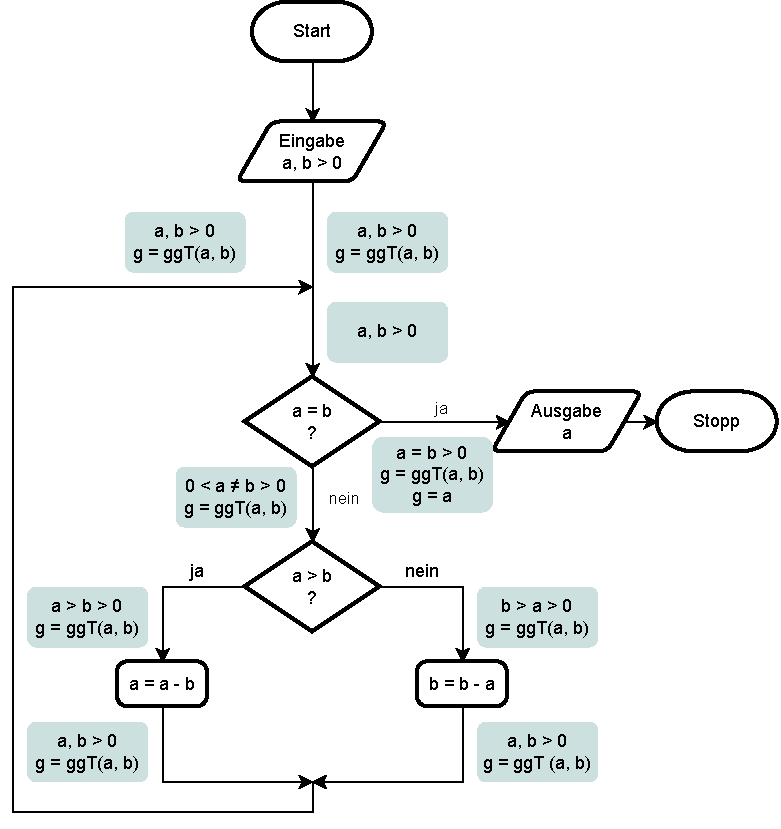
\includegraphics[width=0.9\textwidth]{Bilder/Kapitel-11/Flussdiagramm_Algorithmus_Hoare.pdf}
	\caption{Flussdiagramm mit Zusicherungen}
	\label{fig:flussdiagramm_flgorithmus_hoare}
\end{figure}

Wir betrachten zur Motivation das Flussdiagramm aus Abbildung~\ref{fig:flussdiagramm_flgorithmus_hoare}. Es entspricht dem im vorausgehenden Abschnitt angegebenen Algorithmus~\ref{algo:dritter_reparaturversuch}, also dem letzten Algorithmus zur Berechnung des größten gemeinsamen Teilers zweier Zahlen. Wie kann man verstehen, was dieses Programm macht, ohne seine Abläufe explizit zu betrachten? Wie kann man insbesondere Aussagen zu allen Abläufen machen, obwohl es unendlich viele Abläufe gibt (wir betrachten hier beliebige natürliche Zahlen und beachten nicht, dass kein Rechner unendlich viele unterschiedliche Zahlen darstellen kann)?

Versetzen Sie sich bitte in die Situation, jemand Anderem zu erklären, warum dieses Programm das tut, was es tun soll, also den größten gemeinsamen Teiler der eingegebenen Zahlen $a$ und $b$ bestimmt. Dazu ist es naheliegend, auf gewisse Stellen des Diagramms zu zeigen und anzugeben, was gilt, wenn der Rechner bei der Ausführung „an dieser Stelle ist“. Dafür verwenden wir \emph{Zusicherungen}, 
\marginline{Zusicherungen: Annotationen der Kanten eines Fluss-\\diagramms}
die als \emph{Annotationen} an Kanten geschrieben werden. Diese Beweismethode geht zurück auf Robert Floyd \cite{flo93}.

So wissen wir nach der Eingabe, dass $a > 0$ und $b > 0$ gelten, denn nur dafür ist das Programm gemacht, für andere Eingaben wird nichts gefordert. Deshalb haben wir als erste Annotation an die aus der Eingabe ausgehende Kante diese Eigenschaft von $a$ und $b$ als Zusicherung geschrieben.

Wir verwenden nur für den Zweck der Verifikation eine zusätzliche Variable $g$ (eigentlich eine Konstante), die nicht als Programmvariable zu verstehen ist. Sie enthält das gewünschte Ergebnis laut Spezifikation, also den größten gemeinsamen Teiler von $a$ und $b$. Die später erfolgende Ausgabe sollte dann dem Wert von $g$ entsprechen. Nochmal: $g$ gehört nicht zum Programm und wird auch nicht berechnet, sondern dient hier ausschließlich der Verifikation. Wir können nicht stattdessen $\ggt(a,b)$ verwenden, denn die Werte der Programmvariablen $a$ und $b$ verändern sich während der Programmausführung, und damit potentiell auch $\ggt(a,b)$ (tatsächlich geschieht dies nicht, aber das wird erst zu zeigen sein).

\vspace{1.7mm} %%% für Druck

Anschließend führen zwei Pfeile zusammen, zur ersten Verzweigung $a=b? $ kann man auch über den von links einmündenden Pfeil kommen. Gilt denn auch $a > 0$ und $b > 0$, wenn man von dort kommt? Dies ist zwar der Fall, aber wir können es noch nicht zeigen. Hier kommt nun ein Trick, der mit (den noch einzuführenden) Schleifeninvarianten zusammenhängt: Wir nehmen an, dass auch $a,b > 0$ gilt, wenn wir von links kommen, merken uns aber, dass wir dies später noch begründen müssen.

\vspace{1.7mm} %%% für Druck

Wenn die Bedingung $a = b$ der ersten Verzweigung nicht erfüllt ist, gilt $a < b$ oder $a > b$, sowie weiterhin $a,b >0$. Dies wird an dieser Kante äquivalent und platz\-sparend notiert durch $0<a\neq b >0$. Natürlich gilt weiterhin auch $g = \ggt(a,b)$.

\vspace{1.7mm} %%% für Druck

Die zweite Verzweigung separiert die beiden Fälle $a>b $ und $a<b$, $a=b$ können wir ja hier ausschließen. Links gilt $a > b$, rechts $a < b$. Auf beiden Seiten gilt weiterhin $a,b > 0$.

\vspace{1.7mm} %%% für Druck

Betrachten wir weiter den linken Ast: Da dort $a > b$ gilt, ergibt $a - b$ einen positiven Wert, der $a$ zugewiesen wird. Anschließend gilt also $a > 0$, und natürlich weiterhin $b > 0$. Beim rechten Ast gilt entsprechend ebenfalls nach der Zuweisung $a,b > 0$. Dies gilt also auch nach Zusammenführung der beiden Äste, und die oben „geliehene“ Zusicherung ist damit tatsächlich erfüllt.

\vspace{1.7mm} %%% für Druck

Nun folgt etwas Mathematik. Eine erste Überlegung ist, dass für $a > b$, $\ggt(a,b) = \ggt(a-b,b)$ gilt. Betrachten wir einen gemeinsamen Teiler von $a$ und $b$, also eine Zahl $c$, so dass $a$ und auch $b$ Vielfache von $c$ sind. Dann ist auch $a-b$ Vielfaches von $c$. Umgekehrt gilt: Wenn $a - b$ und $b$ Vielfache von $c$ sind, dann auch $a$ und $b$. Also ist die Menge der gemeinsamen Teiler von $a$ und $b$ identisch mit der Menge der gemeinsamen Teiler von $a - b$ und $b$. Folglich stimmt auch der größte gemeinsame Teiler überein. Entsprechend gilt, für $b > a, \ggt(a,b) = \ggt(a,b-a)$.

\vspace{1.7mm} %%% für Druck

Da $a = a-b$ und $b= b-a$ die einzigen Anweisungen sind, die $a$ oder $b$ verändern, gilt deshalb überall $g = \ggt(a,b)$.

\vspace{1.7mm} %%% für Druck

Eine zweite, einfachere Überlegung ist, dass für $a = b$ gilt: $\ggt(a,b) = \ggt(a,a) = a$. Es gilt $a=b$ beim rechten ausgehenden Pfeil 
der Verzweigung $a=b?$. Daher liefert $a$ den korrekten Wert für $g = \ggt(a,b) = \ggt(a,a) = a$.

\vspace{1.7mm} %%% für Druck

Sind wir mit diesen Überlegungen nun fertig? Tatsächlich lässt sich so zeigen, dass die Ausgabe korrekt ist, wenn sie denn erfolgt. 
\marginline{partielle Korrektheit: jede Ausgabe\\ ist korrekt}
Man nennt diese Eigenschaft \emph{\mbox{partielle} Korrektheit}. Was noch gezeigt werden muss, ist, dass die Ausgabe tatsächlich erreicht wird. Da wir in unserem Programm eine Schleife haben, ist dies ja nicht selbst\-verständlich. Was ist, wenn die Abfrage $a=b?$ stets "`nein"' ergibt und generell, wenn eine Schleife -- für eine bestimmte Eingabe -- nie verlassen wird? Wir nennen eine derartig endlos laufende Schleife \textit{Endlosschleife}.
\marginline{Endlosschleife}

\vspace{1.7mm} %%% für Druck

Wenn wir die partielle Korrektheit bereits gezeigt haben und zusätzlich beweisen können, dass die Ausgabe tatsächlich erreicht wird, dann haben wir die \emph{totale Korrekt\-heit} des Programms bewiesen, und genau das ist unser Ziel. Totale Korrektheit bedeutet, dass die Spezifikation erfüllt ist, wenn wir sie als Zusicherung bei der Ausgabe formuliert haben.

\vspace{1.7mm} %%% für Druck

Wie zeigt man generell, dass eine Schleife irgendwann einmal verlassen wird? Dafür verwendet man meist eine sogenannte \emph{Abstiegsfunktion}. 
\marginline{Abstiegs\-funktion}
Dies ist eine Abbildung der Variablen des Programms auf die natürlichen Zahlen mit der Eigenschaft, dass der Funktionswert bei jedem Schleifendurchlauf abnimmt. Zusätzlich muss gezeigt werden, dass dieser Wert nicht beliebig klein werden kann (so wie es auch keine beliebig kleinen natürlichen Zahlen gibt), also spätestens beim Wert 0 die Schleife verlassen wird. Natürlich hängt diese Abstiegsfunktion stets nur von den Variablenwerten ab, die in der Schleife verändert werden.

\vspace{1.7mm} %%% für Druck

In unserem Beispiel lautet eine geeignete Abstiegsfunktion $f(a,b) = a+b$. Da die Werte von $a$ und $b$ stets positiv bleiben, wird $f(a,b)$ sowohl bei der Anweisung $a = a-b$ als auch bei der Anweisung $b = b-a$ kleiner. Eine der beiden Anweisungen kommt aber bei jedem Schleifendurchlauf vor. Ebenfalls weil $a$ und $b$ stets positiv bleiben, gilt dies für $f(a,b)$. Tatsächlich ist der kleinstmögliche Wert 2, nämlich für $a = b = 1$. Spätestens in diesem Fall wird die Schleife aber verlassen und es wird 1 ausgegeben. Die beiden Eingabewerte waren in diesem Fall teilerfremd. Natürlich kann die Schleife gegebenenfalls auch früher, \dasHeisst bei größeren Werten von $f(a,b)$ verlassen werden.
\subsection{Partielle Korrektheit}
\label{sec:Kap-11-2-2}

Die Ideen von Robert Floyd zu Zusicherungen an Kanten von Flussdiagrammen wurden von Tony Hoare für Programmcode übernommen und weiter formalisiert \cite{hoa69}. 

\vspace{1.7mm} %%% für Druck

Bekannt geworden sind sogenannte \emph{Hoare-Tripel}
\marginline{Hoare-Tripel}

\vspace{\baselineskip} %%% für Druck

$$\text{ \{Vorbedingung\} \;\; Programm \;\; \{Nachbedingung\} }$$

\vspace{\baselineskip} %%% für Druck

mit der Bedeutung: Wenn die \emph{Vorbedingung} erfüllt ist und das Programm ausgeführt wird, ist anschließend die \emph{Nachbedingung} erfüllt. Die Vor- und Nachbedingungen werden hier auch Zusicherungen genannt. Sie haben Hoare-Tripel bereits in der vorhergehenden Lektion kennengelernt. Hier benötigen (und definieren) wir sie wieder und verwenden sie in einem noch formaleren Kontext. Wichtig ist, dass ein Hoare-Tripel nichts dazu sagt, was gilt, wenn die Vorbedingung vor Ausführung des Programms nicht erfüllt ist. Wichtig ist zudem, dass die Nachbedingung nur erfüllt sein muss, wenn das Programm tatsächlich vollständig ausgeführt wurde. Bei einer Endlosschleife zum Beispiel gilt das Hoare-Tripel ebenfalls als erfüllt. Statt „erfüllt“ sagt man auch „gültig“.

Das Programm ist \emph{partiell korrekt}, wenn für jede gültige Eingabe (die die Vorbedingung erfüllt) jede Ausgabe die Nachbedingung erfüllt. In die Nachbedingung muss man also die Spezifikation hineincodieren, oft in Bezug auf die Vorbedingung.

Um die partielle Korrektheit eines Programms zu beweisen, betrachtet man einzelne Programmstücke, in diesem Kontext auch \textit{Segmente} genannt, und viele Zusicherungen innerhalb des Programms. Für jedes Segment $S$, das von einzelnen Anweisungen bis hin zu dem vollständigen Programm gehen kann, werden dann Hoare-Tripel $\{P\} \; S \; \{Q\}$ betrachtet bzw. im mathematischen Sinne als gültig bewiesen. Der eigentliche Clou bei diesem sogenannten \emph{Hoare-Kalkül} 
\marginline{Hoare-Kalkül}
ist, dass man gültige Hoare-Tripel aus anderen Hoare-Tripeln ableiten kann, das heißt (fast) rein syntaktisch und damit auch für einen Rechner leicht nachprüfbar herleiten kann.

\vspace{\baselineskip} %%% für Druck

\sttpAutorenkasten{Tony Hoare}{1934}{}{Britischer Informatiker. Entwickelte den Quicksort-Algo\-rith\-mus, das Hoare-Kalkül sowie die Prozessalgebra CSP. Erhielt 1980 den Turing Award. Emeritierter Professor der Universität Oxford.}{Bilder/Autoren/hoare.jpg}{2011}{Rama, \href{https://creativecommons.org/licenses/by-sa/2.0/fr/deed.en}{CC BY-SA 2.0 FR}, via \href{https://commons.wikimedia.org/wiki/File:Sir_Tony_Hoare_IMG_5123.jpg}{Wikimedia Commons}}

\vspace{\baselineskip} %%% für Druck

Betrachten wir zunächst eine Zuweisung $x = e$, wobei $x$ eine Variable und $e$ ein Ausdruck ist, in dem auch Variablen (möglicherweise auch $x$) samt Operatoren vorkommen können. Es sollte klar sein, was sich durch Ausführung dieser Anweisung verändert, sofern man von Funktionsaufrufen, Nebeneffekten usw. absieht: Der Wert des Ausdrucks $e$ wird ermittelt und der Variable $x$ zugewiesen. Insbesondere ändert sich ausschließlich der Wert von $x$. Das heißt aber, dass alle Zusicherungen, die $x$ nicht betreffen und vor Ausführung der Zuweisung gelten, auch danach gelten, also nicht verändert werden. Nach der Zuweisung gelten alle Aussagen für die Variable $x$, die vorher für den Ausdruck $e$ galten.

Sehen wir uns ein Beispiel an: Unsere Vorbedingung sei $\{y > z\}$ und der Befehl, den wir betrachten, sei $x = y + 1$. Der Ausdruck $e$ ist also $y + 1$. Was gilt laut Vorbedingung für $y+1$? Aus $y > z$ folgt $y + 1 > z + 1$. Also gilt nach der Ausführung die Nachbedingung $\{x > z + 1\}$ und natürlich immer noch $\{y>z\}$, denn $y$ und $z$ wurden ja nicht verändert. Tatsächlich erhält man die Nachbedingung $\{x > z + 1\}$ aus $\{ y + 1 > z + 1\}$, in dem man syntaktisch (!) die Zeichenkette „$y+1$“, also den Ausdruck $e$, durch das Zeichen $x$ ersetzt.

Das generelle Vorgehen lautet wie folgt: Wir führen eine logische Umformung der Vorbedingung aus, so dass der Ausdruck (hier $e$) als Teilterm vorkommt und ersetzen diesen durch das Variablensymbol (hier $x$). Natürlich reicht eine Implikation für die logische Umformung aus, denn wenn $P$ gilt und zugleich $P \Rightarrow Q$ gilt, dann gilt \mbox{auch $Q$}.

Formal verwendeten wir bis hierhin bereits zwei Regeln, die im Hoare-Kalkül durch Angabe von Prämissen (Voraussetzungen, über dem Strich) und Konklusion (Folgerung, unter dem Strich) wie folgt notiert werden:

\minisec{Konsequenzregel}

\vspace{2mm} %%% für Druck

$$\frac{P'\Rightarrow P \quad \{P\}\; S\; \{Q\}\quad Q \Rightarrow Q'}{\{P'\}\; S\; \{Q'\}}$$ 

\minisec{Zuweisungsregel}

$$\frac{}{\{P[x/e]\} \quad x = e \quad \{P\}}$$

Die Zuweisungsregel hat also keine Prämisse. $[x/e]$ entspricht dem syntaktischen Ausdruck für $P$, in dem alle Vorkommen von $x$ durch $e$ ersetzt werden.

Die weiteren Regeln folgen nun dem Aufbau der Programmstruktur. Wir betrachten hier der Einfachheit halber eine primitive Programmiersprache, die nur die \mbox{Strukturen}
\begin{itemize}
	\item Sequenz ($S$; $S'$),
	\item Verzweigung (\textbf{if} $B$ \textbf{then} $S$ \textbf{else} $S'$)
	\item Schleife (\textbf{while} $B$ \textbf{do} $S$)
\end{itemize}

kennt. Damit kann man allerdings grundsätzlich bereits alle Algorithmen darstellen.

\minisec{Sequenzregel}

\vspace{2mm} %%% für Druck


$$\frac{\{P\} \; S \; \{Q\} \quad \{Q\} \; S' \; \{R\}}{\{P\} \; S;S' \; \{R\}}$$

Die Korrektheit dieser Regel ist recht offensichtlich. Angenommen: Wenn $P$ gilt und das Programmsegment $S$ ausgeführt wird, gilt anschließend $Q$, und wenn $Q$ gilt und das Programmsegment $S'$ ausgeführt wird, gilt anschließend $R$. Dann können wir bei Vorliegen von $P$ die Segmente $S$ und $S'$ nacheinander ausführen, und es gilt anschließend $R$.

\minisec{Verzweigungsregel}

\vspace{2mm} %%% für Druck

$$\frac{\{P \wedge B\} \; S \; \{Q\} \quad \{P \wedge \neg B\} \; S' \; \{Q\}}{\{P\} \; \textbf{if} \; B \; \textbf{then} \; S \; \textbf{else} \; S' \; \{Q\}}$$

Auch hier ist die Korrektheit leicht zu begründen. Dieses Programmsegment besteht aus den beiden Alternativen $S$ und $S'$, die je nach Auswertung der Bedingung $B$ ausgeführt werden. Gilt $B$, wird $S$ ausgeführt, und wir können für $S$ natürlich $B$ als zusätzliche Vorbedingung verwenden. Gilt $B$ dagegen nicht, wird $S'$ mit zusätzlicher Vorbedingung $\neg B$ ausgeführt. Es gehört zur Prämisse außerdem, dass in beiden Fällen anschließend $Q$ gilt. Also gilt dies auch für das gesamte Programmsegment.

\minisec{Schleifenregel}

\vspace{2mm} %%% für Druck

$$\frac{\{P \wedge B\} \; S \; \{P\}}{\{P\} \; \textbf{while} \; B \; \textbf{do} \; S \; \{P \wedge \neg B\} }$$

\vspace{2mm} %%% für Druck

Die Prämisse sagt etwas über den Schleifenrumpf $S$ aus: Wir betrachten eine Bedingung $P$, die vor und nach der Ausführung von $S$ gilt. Diese Bedingung heißt \emph{Schleifen\-invariante}, 
\marginline{Schleifen\-invariante}
denn sie wird durch den gesamten Schleifenrumpf nicht verändert. Es kann aber durchaus sein (und ist meist so), dass $P$ nach nur teilweiser Ausführung von $S$ nicht mehr gilt. Es kommt nur darauf an, dass die Schleifen\-invariante $P$ nach vollständiger Abarbeitung von $S$ gilt. Als zusätzliche Vorbedingung können wir bei der Prämisse $B$ annehmen. Hier nutzen wir aus, dass die Schleife nur bei Gültigkeit von $B$ betreten wird.

\vspace{2mm} %%% für Druck

Nehmen wir nun an, dass die Schleife etliche Male durchlaufen wurde und schließlich verlassen wird. Dann gilt jedenfalls $\neg B$, denn sonst würde sie ja nicht verlassen. Und es gilt aufgrund der Prämisse weiterhin $P$, denn zu jedem Ende eines Schleifendurchlaufs, also auch des letzten Schleifendurchlaufs, wurde $P$ ja wiederhergestellt. Wird die Schleife gar nicht durchlaufen, weil gleich $\neg B$ gilt, ist die Nachbedingung der Konklusion natürlich auch erfüllt. Wenn die Schleife allerdings niemals verlassen wird, gilt auch niemals nach Beendigung des Schleifenrumpfs $\neg B$ und die Nachbedingung insgesamt wird nicht erfüllt. Die Regel ist in diesem Fall dennoch korrekt, denn sie sagt ja nur etwas darüber aus, welche Nachbedingungen nach Beendigung eines Programmsegments erfüllt sind.

\vspace{2mm} %%% für Druck

Die Schleifeninvariante sieht formal so unschuldig aus, doch ist das Finden geeigneter Schleifeninvarianten für die erfolgreiche Verifikation eines Programms mit Schleifen manchmal gar nicht so leicht. Man sagt umgekehrt, dass man eine geeignete Schlei\-fen\-in\-va\-ri\-ante dann und nur dann findet, wenn man die Idee des Programms und seiner Schleifenstruktur vollständig verstanden hat.

\vspace{2mm} %%% für Druck

Wir schreiben nun das bereits verwendete Beispielprogramm zur Bestimmung des ggT zweier positiver Zahlen vollständig mit Zusicherungen auf (s.~Algorithmus~\ref{algo:berechnung_ggt_mit_zusicherungen}). Manche Variablen sind Programmvariablen (hier $a$ und $b$), andere zusätzliche 
\linebreak %%% für Druck
Variablen (hier $g$).

\vspace{-2mm}

\begin{algorithm}
	\caption{Algorithmus zur Berechnung des ggT von $a$ und $b$ mit Zusicherungen}
	\label{algo:berechnung_ggt_mit_zusicherungen}
	
	\vspace{2mm} %%% für Druck
	\vspace{\baselineskip}
	
	\KwData{Eingabe: $a, b > 0$}
	\KwResult{Ausgabe: $\ggt(a,b)$}
	
	\vspace{2mm} %%% für Druck
	\vspace{\baselineskip}
	
	\HiLi $\{a > 0, \, b > 0, \, g = \ggt(a,b)\}$ \\
	
	\vspace{2mm} %%% für Druck
	\vspace{\baselineskip}
	
	\While{$a \neq b$}
	{
		\vspace{2mm} %%% für Druck
		\vspace{\baselineskip}
		
		\HiLi $\{a > 0, \, b > 0, \, a \neq b, \, g = \ggt(a,b)\}$ \\
		
		\vspace{2mm} %%% für Druck
		\vspace{\baselineskip}
		
		\eIf{$a > b$}{
			\HiLi $\{a > b > 0, \, g = \ggt(a,b)\}$ \\
			\HiLi $\{a - b > 0, \, b > 0, \, g = \ggt(a-b,b)\}$ \\
			\vspace{\baselineskip} %%% für Druck
			$a = a - b$ \\
			\vspace{\baselineskip} %%% für Druck
			\HiLi $\{a > 0, \, b > 0, \, g = \ggt(a,b)\}$
		}{
			\HiLi $\{a \neq b, \, 0 < a \leq b, \, g = \ggt(a,b)\}$ \\
			\HiLi $\{0 < a < b, \, g = \ggt(a,b)\}$ \\
			\HiLi $\{b - a > 0, \, a > 0, \, g = \ggt(a,b-a)\}$ \\
			\vspace{\baselineskip} %%% für Druck
			$b = b - a$ \\
			\vspace{\baselineskip} %%% für Druck
			\HiLi $\{b > 0, \, a > 0, \, g = \ggt(a,b)\}$
		}
	}
	\;
	
	\vspace{2mm} %%% für Druck
	\vspace{\baselineskip}
	
	\HiLi $\{a = b, \, a > 0, \, b > 0, \, g= \ggt(a,b)\}$ \\
	\HiLi $\{g = a\}$
	
	\vspace{2mm} %%% für Druck
	\vspace{\baselineskip}
	
	\Return{$a$}

	\vspace{2mm} %%% für Druck
	\vspace{\baselineskip}
\end{algorithm}

\clearpage %%% für Druck

Unter Anwendung der genannten Regeln können wir nachweisen, dass das Programm, wenn überhaupt, mit der Ausgabe $a$ terminiert, die den gesuchten Wert $g$ hat. Dies macht man von innen nach außen; wir beginnen mit der Zuweisungs\-regel für die beiden Zuweisungen, wenden dann die Verzweigungsregel und schließlich die Schleifenregel an. Die erforderlichen Zusicherungen lassen sich allerdings kaum von innen nach außen erraten, hierfür sollte man die Logik des Programms und ins\-besondere der Schleife gut verstehen.

\vspace{2mm} %%% für Druck

Bevor wir in den nächsten Abschnitten zwei weitere Beispiele für die Anwendung des Hoare-Kalküls angeben werden, wollen wir die Frage beantworten, ob wir jedes korrekte Programm tatsächlich auf diesem Wege verifizieren können. Im Grunde hieße dies, dass wir stets eine geeignete Schleifeninvariante angeben können und entsprechend das Programm mit Zusicherungen annotieren können, so dass mit Hilfe der Hoare'schen Regeln die Korrektheit syntaktisch nachprüfbar ist. Die Antwort darauf ist etwas komplex: Ja, das Hoare-Kalkül ist vollständig, und jedes korrekte Programm (der hier verwendeten Sprache) lässt sich auf diesem Weg verifizieren. Ein guter Teil einer Verifikation mag allerdings in der Logik versteckt sein: Unsere erste Regel, die Konsequenzregel, verwendet als Prämisse Implikationen $P' \Rightarrow P$ und $Q \Rightarrow Q'$. Da $P, P'$ bzw. $Q, Q'$ komplexe logische Ausdrücke sein können und die Gültigkeit der Implikation nicht in jeder Logik durch Anwendung syntaktischer Regeln nachgewiesen werden kann, ist hier auch eine grundsätzliche Schranke für die rein syntaktische Verifikation verborgen. Dies betrifft aber nicht die Regeln, die sich auf die Struktur eines Programms beziehen.
\vspace{2mm} %%% für Druck

\subsection{Beispiel: Fibonacci-Zahlen}
\label{sec:Kap-11-2-3}

Die Fibonacci-Zahlen $f_1, f_2, f_3, \ldots $ sind wie folgt definiert: $f_1 = 1, f_2 = 1$ und, für $i \geq 3$, $f_i = f_{i-2} + f_{i-1}$. Die ersten sieben Fibonacci-Zahlen lauten daher

$$f_1=1, f_2=1, f_3=2, f_4=3, f_5=5, f_6=8, f_7=13 $$

Algorithmus~\ref{algo:fibonacci} gibt einen bereits mit Zusicherungen annotierten Algorithmus zur Berechnung der $k$-ten Fibonacci-Zahl an, wobei $k \geq 2$ die Eingabe darstellt.

%%% Hier kommt Algorithmus "algo:fibonacci" eigentlich hin.

\vspace{2mm} %%% für Druck

Die Schleifeninvariante lautet in diesem Beispiel also

$$\{n=f_{i-2} \wedge m= f_{i-1} \wedge i \leq k+1\}.$$ 

Der Teil $i \leq k+1$ ist etwas lästig und hätte vermieden werden können, wenn die Schleifenabbruchbedingung $i \neq k + 1 $ gelautet hätte, doch wir wollten es Ihnen nicht zu einfach machen :-). Nun funktioniert der Algorithmus auch für die Eingabe $k=1$, die Verifikation mit den angegebenen Zusicherungen allerdings nicht. Was müsste geändert werden, um die Korrektheit auch für diesen Fall zu zeigen? Tatsächlich wird diese Verallgemeinerung recht umständlich, so dass man diesen einen Fall gesondert zeigen kann: Die Schleife wird nicht betreten und der korrekte Wert $m= 1$ wird ausgegeben.

\begin{algorithm}
	\caption{Algorithmus zur Berechnung der $k$-ten Fibonacci-Zahl}
	\label{algo:fibonacci}
	
	\vspace{\baselineskip}
	
	\KwData{Eingabe: $k, k \geq 2$}
	\KwResult{Ausgabe: $f_k$}
	
	\vspace{\baselineskip}
	
	$n = 1; \, m = 1; \, i = 3;$ \\
	
	\HiLi $\{n = f_{i-2}, \, m = f_{i-1}, \, i \leq k+1\}$ \\
	
	\vspace{\baselineskip}
	
	\While{$i \leq k$}{
		\HiLi $\{i \leq k, \, n = f_{i-2}, \, m = f_{i-1}\}$ \\
		\HiLi $\{m + n = f_{i-2} + f_{i-1}\}$ \\
		\vspace{\baselineskip} %%% für Druck		
		$m = m + n$\;
		\vspace{\baselineskip} %%% für Druck		
		\HiLi $\{i \leq k, \, n = f_{i-2}, \, m = f_{i-2} + f_{i-1}\}$ \\
		\HiLi $\{m - n = f_{i-1}\}$ \\
		\vspace{\baselineskip} %%% für Druck		
		$n = m - n$\;
		\vspace{\baselineskip} %%% für Druck		
		\HiLi $\{i \leq k, \, n = f_{i-1}, \, m = f_{i-2} + f_{i-1}= f_i\}$ \\
		\HiLi $\{i+1 \leq k+1, \, n = f_{i+1 - 2}, \, m = f_{i+1 - 1}\}$ \\
		\vspace{\baselineskip} %%% für Druck		
		$i = i + 1$ \\
		\vspace{\baselineskip} %%% für Druck		
		\HiLi $\{i \leq k+1, \, n = f_{i-2}, \, m = f_{i - 1}\}$ \\
	}
	\;
	
	\vspace{\baselineskip}
	
	\HiLi $\{i > k, \, i \leq k+1, \, n = f_{i-2}, \, m = f_{i-1}\}$ \\
	\HiLi $\{i = k+1\}$ \\
	\HiLi $\{m = f_k\}$\\
	
	\vspace{\baselineskip}
	
	\Return{$m$}
	
	\vspace{\baselineskip}
	
\end{algorithm}
\clearpage %%% für Druck

\subsection{Beispiel: Multiplikation durch Halbieren}
\label{sec:Kap-11-2-4}

Die Multiplikation zweier natürlicher Zahlen wird üblicherweise durch fortgesetzte Addition eingeführt: $a \cdot b$ entsteht durch $b$-malige Addition von $a$ (beginnend mit 0) oder $a$-malige Addition von $b$. Sind beide Zahlen relativ groß, ist dies nicht sonderlich effizient.

\vspace{2mm} %%% für Druck

Es geht deutlich schneller, wenn man sich die Binärdarstellung natürlicher Zahlen zunutze macht. Sie erlaubt die ganz einfache Multiplikation einer Zahl mit 2, nämlich durch Anhängen einer 0, sowie die Division durch 2 ohne Rest durch Wegnahme der letzten binären Ziffer. Technisch wird dasselbe etwas anders realisiert: statt Anhängen einer 0 werden alle Bits einer Variablen um eine Stelle nach links verrutscht, und statt Wegnehmen der letzten Stelle werden alle Bits um eine Stelle nach rechts verrutscht. Entsprechende Shift-Operationen auf Registerebene stehen in Maschinensprachen zur Verfügung. Wir gehen an dieser Stelle einmal davon aus, dass alle betrachteten Zahlen und Produkte nicht zu einem Überlauf führen, also die Variablenbereiche ausreichend groß dimensioniert sind. 

\vspace{2mm} %%% für Druck

Zudem kann man sehr einfach feststellen, ob eine Zahl ungerade ist, nämlich durch Prüfung des geringstwertigen Bits. Im Folgenden bezeichne $n \, \text{DIV} \, 2$ die Division einer Zahl $n$ durch 2 ohne Rest und $\text{odd}(n)$ prüft, ob $n$ ungerade ist.

\vspace{2mm} %%% für Druck

Betrachten Sie zunächst das folgende Programm ohne Zusicherungen und überlegen Sie sich, wie die Schleifeninvariante aussehen könnte:

\vspace{\baselineskip}

\begin{algorithm}[H]
	\caption{Multiplikation durch Halbieren}
	\label{algo:multiplikation_durch_halbieren_1}
	
	\vspace{\baselineskip}
	
	\KwData{Eingabe: $n,m \geq 1$}
	\KwResult{Ausgabe: $n \cdot m$}
	
	\vspace{\baselineskip}
	
	$p = 0$\;
	
	\vspace{\baselineskip}
	
	\While{$n \neq 1$}{
		
		\vspace{\baselineskip}
		
		\If{$\text{odd}(n)$}
		{
			$p = p + m$
		}
		
		\vspace{\baselineskip}
		
		$n = n \, \text{DIV} \, 2$\;
		$m = m \cdot 2$
	}
	\;
	
	\vspace{\baselineskip}
	
	\Return{$p + m$}
	
	\vspace{\baselineskip}
	
\end{algorithm}

\vspace{\baselineskip}
\vspace{\baselineskip} %%% für Druck

Und nun das vollständig annotierte Programm:

\pagebreak %%% für Druck

\begin{algorithm}
	\caption{Multiplikation durch Halbieren mit Zusicherungen}
	\label{algo:multiplikation_durch_halbieren_2}
	
	\vspace{\baselineskip}
	
	\KwData{Eingabe: $n,m \geq 1$}
	\KwResult{Ausgabe: $n \cdot m$}
	
	\vspace{\baselineskip}
	
	\HiLi $\{n \geq 1, \, m \geq 1\}$ \\
	\HiLi $\{e = n \cdot m\}$ \quad \tcc*[h]{\small $e$ ist keine Programmvariable,}\\
	~~~~~~~~~~~~~~~~\quad \tcc*[h]{\small ihr Wert ist das gewünschte Ergebnis}\
	
	$p = 0$\;
	\HiLi $\{n \geq 1, \, m \geq 1, \, p = 0, \, e = n \cdot m\}$ \\
	\HiLi $\{n \cdot m + p = e\}$ \\
	
	\vspace{\baselineskip}
	
	\While{$n \neq 1$}{
		\HiLi $\{n \cdot m + p = e\}$ \\
		
		\vspace{\baselineskip}
		
		\eIf{$\text{odd}(n)$}{
			\HiLi $\{n \cdot m + p = e, \, (n \, \text{DIV} \, 2) \cdot 2 + 1 = n\}$ \\
			\HiLi $\{[(n \, \text{DIV} \, 2) \cdot 2 + 1] \cdot m + p = e\}$ \\
			\HiLi $\{(n \, \text{DIV} \, 2) \cdot 2 \cdot m + p + m = e\}$ \\
			\vspace{\baselineskip} %%% für Druck
			$p = p + m$ \\
			\vspace{\baselineskip} %%% für Druck
			\HiLi $\{(n \, \text{DIV} \, 2) \cdot 2 \cdot m + p = e \}$
		}{
			\HiLi $\{n \cdot m + p = e, \, (n \, \text{DIV} \, 2) \cdot 2 = n\}$ \\
			\HiLi $\{(n \, \text{DIV} \, 2) \cdot 2 \cdot m + p = e\}$
		}
		
		\vspace{\baselineskip}
		
		\HiLi $\{(n \, \text{DIV} \, 2) \cdot 2 \cdot m + p = e\}$ \\
		\vspace{\baselineskip} %%% für Druck
		$n = n \, \text{DIV} \, 2$\;
		\vspace{\baselineskip} %%% für Druck
		\HiLi $\{n \cdot 2 \cdot m + p = e\}$ \\
		\HiLi $\{n \cdot m \cdot 2 + p = e\}$ \\
		\vspace{\baselineskip} %%% für Druck
		$m = m \cdot 2$ \\
		\vspace{\baselineskip} %%% für Druck
		\HiLi $\{n \cdot m + p = e\}$
	}
	\;
	
	\vspace{\baselineskip}
	
	\HiLi $\{n \cdot m + p = e, \, n = 1\}$ \\
	\HiLi $\{p + m = e\}$ \\ 
	
	\vspace{\baselineskip}
	
	\Return{$p + m$}
	
	\vspace{\baselineskip}
	
\end{algorithm}

\clearpage %%% für Druck

Hier mussten wir etwas umständlich codieren, dass $n$ eine ungerade Zahl ist. Dies haben wir durch $n \, \text{DIV} \, 2$ ausgedrückt, denn dieser Ausdruck kommt bei einer Zuweisung auf der rechten Seite vor. Für ungerade Zahlen $n$ gilt $(n \, \text{DIV} \, 2) \cdot 2 = n-1$ und für gerade $n$ gilt $(n \, \text{DIV} \, 2) \cdot 2 = n$.

Auch hier stellt sich natürlich die Frage, ob und warum das Programm terminiert, also die Ausgabe überhaupt erreicht. Als Abstiegsfunktion bietet sich die Variable $n$ an, denn sie wird stets kleiner. Für $n=1$ bricht die Schleife ab, und kleiner als 1 kann $n$ durch Halbierung einer Zahl, die größer als 1 ist, nicht werden.
\subsection{Totale Korrektheit}
\label{sec:Kap-11-2-5}

\minisec{Terminierung von Schleifen}

Wir haben in den Beispielen oben bereits gezeigt, dass die jeweiligen Schleifen tatsächlich terminieren. Dazu haben wir Abstiegsfunktionen angegeben, also Funktionen mit Argumenten aus den Variablen, die im Schleifenrumpf modifiziert werden können. Die Werte einer Abstiegsfunktion dürfen nicht beliebig klein werden, und sie müssen bei jedem Schleifendurchlauf kleiner werden. Typischerweise wird bei dem kleinstmöglichen Wert die Schleife verlassen, aber oftmals kann die Schleife auch bei größeren Werten verlassen werden.

Aber Vorsicht, die fortgesetzte Halbierung einer Zahl führt auch zu einer immer kleiner werdenden Zahl, ohne dass die 0 jemals erreicht wird. Deshalb betrachtet man nur ganzzahlige Abstiegsfunktionen, \dasHeisst der Wert reduziert sich bei jedem Schleifendurchlauf um wenigstens 1.

Abstiegsfunktionen sind nicht immer offensichtlich oder leicht zu finden. Betrachten Sie als Beispiel folgendes Programm:

\vspace{\baselineskip} %%% für Druck

\begin{algorithm}[H]
	\caption{$n+1$-Programm}
	\label{algo:n_plus_1_programm}
	
	\vspace{2mm} %%% für Druck
	\vspace{\baselineskip}
	
	\KwData{Eingabe: $n > 0$}
	\KwResult{Ausgabe: $m$}
	
	\vspace{2mm} %%% für Druck
	\vspace{\baselineskip}
	
	$m = 0$\;
	
	\vspace{2mm} %%% für Druck
	\vspace{\baselineskip}

	\While{$n > 1$}{
		\eIf{\text{odd}($n$)}{
			$n = n + 1$
		}{
			$n = n / 2$
		}
		$m = m + 1$
	}
	\;
	
	\vspace{2mm} %%% für Druck
	\vspace{\baselineskip}
	
	\Return{$m$}
	\vspace{2mm} %%% für Druck
	\vspace{\baselineskip}
\end{algorithm}

\pagebreak %%% für Druck

Auf die Ausgabe $m$ kommt es hier gar nicht an, sondern uns interessiert nur, dass und warum die Schleife sicher irgendwann verlassen wird. Für verschiedene Anfangswerte ($n = 5, 12, 13$) erhalten wir die folgenden Zahlenfolgen für $n$:

\begin{center}
	$5, 6, 3, 4, 2, 1$ \\
	$12, 6, 3, 4, 2, 1$ \\
	$13, 14, 7, 8, 4, 2, 1$
\end{center}

Aber was steigt hier ab?

Bevor Sie sich die Lösung ansehen, versuchen Sie doch selbst herauszufinden, wie eine für dieses Programm passende Abstiegsfunktion aussehen könnte.

$\vdots$

Und hier ist eine mögliche Lösung:

$$ f: \{1,2,3, \ldots\} \rightarrow \{0,1,2, \ldots \}, \quad f(n) =
\begin{cases}
	0 & \text{für } n = 1 \\
	n - 1 & \text{für } n \text{ gerade} \\
	n + 1 & \text{für } n \text{ ungerade, } n > 1
\end{cases}$$


Die Folge der Funktionswerte für die Argumente $1,2,3,4,5,6,7,8, \ldots$ lautet damit

$$ 0,1,4,3,6,5,8,7, \ldots $$

Nun ist zu zeigen, dass es sich tatsächlich um eine Abstiegsfunktion handelt, bei jedem Schleifendurchlauf der Funktionswert also um wenigstens 1 kleiner wird. Zu beachten ist, dass die Schleife für $n= 1$ verlassen wird, wir also nur die Fälle $n > 1$ betrachten müssen.

\vspace{\baselineskip}

\begin{addmargin}[25pt]{25pt}
\begin{labeling}{{\textbf{xx. Fall:}}} % "xx. Fall" ist hier nur ein Platzhalter
	\item[\textbf{1. Fall:}] $n$ ist eine ungerade Zahl \\
		Dann ist $n \geq 3$. $n$ wird um 1 erhöht. Nach Konstruktion von $f$ gilt $f(n+1) = n = f(n)-1$, der Wert von $f(n)$ wird also kleiner.
	\item[\textbf{2. Fall:}] $n$ ist eine gerade Zahl, $n/2$ ist ebenfalls eine gerade Zahl \\
		$n$ wird im Schleifendurchlauf halbiert. Es gilt $f (n) = n-1 $ und $f(n/2) = n/2 -1$. Der Wert von $f(n)$ wird also um $n/2$ kleiner.
	\item[\textbf{3. Fall:}] $n$ ist eine gerade Zahl, $n/2$ ist eine ungerade Zahl, $n \neq 2$ \\
		Es gilt $f(n) = n-1$ und $f(n/2) = n/2 +1$. Der Wert von $f(n)$ wird also um $n/2 - 2$ reduziert. Dieser Wert ist positiv, da nach Voraussetzung $n\geq 6$ gilt ($n=2$ ist ausgeschlossen, für $n= 4$ ist $n/2$ gerade).
	\item[\textbf{4. Fall:}] $n=2$ \\
		Dann gilt $f(n)= f(2)= 1$. $n$ wird um 1 reduziert und 
		\linebreak
		$f(1) = 0<1$.
\end{labeling}
\end{addmargin}

\vspace{\baselineskip}

Der Funktionswert $f(n)$ wird also in jedem Fall bei jedem Schleifendurchlauf um wenigstens 1 reduziert, weshalb $f$ eine hier passende Abstiegsfunktion darstellt.

In den meisten Fällen sind Abstiegsfunktionen allerdings offensichtlicher, aber nicht immer! Vielleicht macht es Ihnen Spaß, Variationen dieses Beispiels zu untersuchen. Was gilt, wenn ungerade $n$ nicht um 1, sondern um 3 erhöht werden (und gerade $n$ weiterhin halbiert werden)? Eine andere Variation: Bei ungeradem $n$ wird $n$ durch $3n + 1$ ersetzt. Für einen Anfangswert $n=17$ entsteht dann die Zahlenfolge

$$ 17, 52, 26, 13, 40, 20, 10, 5, 16, 8, 4, 2, 1$$

Aber endet diese Folge für jeden beliebigen Anfangswert von $n$, und wie lautet eine entsprechende Abstiegsfunktion? Wenn Sie hier eine akzeptable Antwort finden, werden Sie reich und berühmt. Es handelt sich nämlich um das bekannte Collatz-Problem 
\marginline{Collatz-Problem}
(auch $(3n+1)$-Problem genannt). Man hat weder jemals eine Anfangszahl gefunden, für die diese Schleife nicht terminiert, noch eine Abstiegsfunktion oder irgendeinen anderen Beweis dafür, dass die Schleife immer terminiert.

\minisec{Terminierung bei Rekursion}

Für nicht terminierende Programme braucht man nicht notwendigerweise Schleifen, die sich als Endlosschleifen herausstellen! Derselbe Effekt eines immer weiter laufenden Programms, das nicht zum Ende kommt, taucht auch auf, wenn sich ein Programm (oder eine programmierte Funktion) immer wieder selbst aufruft. Unser letztes Beispiel aus Algorithmus~\ref{algo:n_plus_1_programm} könnte man auch rekursiv programmieren durch

\vspace{\baselineskip}

\begin{algorithm}[H]
	\caption{fun function}
	\label{algo:fun_function}
	
	\vspace{\baselineskip}
	
	\KwData{Eingabe: $n$}
	\KwResult{Ausgabe: None}
	
	\vspace{\baselineskip}
	
	\SetKwFunction{Function}{fun}
	\SetKwProg{Fn}{Function}{:}{end}
	
	\vspace{\baselineskip}
	
	\Fn{\Function{$n$}}{
		\eIf{$n = 1$}{
			\text{stopp}
		}{
			\eIf{\text{odd}($n$)}{
				$\Function(n+1)$
			}{
				$\Function(n/2)$
			}
		}
	}
	
	\vspace{\baselineskip}
\end{algorithm}

\vspace{\baselineskip}

Hätte die Funktion nicht wenigstens einen Fall, in dem sie sich nicht wieder selbst aufruft (hier der Fall $n=1$), dann würden die Selbstaufrufe unweigerlich kein Ende finden. Aber auch wenn es die Möglichkeit eines Endes gibt, ist noch nicht gewährleistet, dass dieses Ende jemals erreicht wird. Notwendig dafür ist, dass das Argument, mit dem die Funktion sich selbst aufruft, kleiner wird, oder eine weniger komplexe Struktur besitzt oder dass es irgendeinen anderen Grund gibt, dass die Abbruch\-bedingung jemals erreicht wird. Hier kann man wie bei Schleifen eine Abstiegsfunktion\footnote{Vorsicht, die doppelte Verwendung von „Funktion“ als Programmelement einerseits und als Abstiegsfunktion andererseits mag verwirren!} $f$ verwenden. Wenn die (Programm-)Funktion mit Argument $n$ aufgerufen wird, darf sie sich selbst nur mit Argumenten $n'$ aufrufen, für die $f(n') < f(n)$ gilt. Die Abstiegsfunktion muss ganzzahlige Werte haben, und diese Werte dürfen nicht beliebig klein werden. Bei einem bestimmten kleinen Wert für $f(n)$ ruft sich die (Programm-)Funktion nicht wieder selbst auf, sondern terminiert; dann kann die aufrufende Instanz der Funktion ebenfalls terminieren, usw.

Bei rekursiven Aufrufen muss man also besonders aufpassen, dass die verwendeten Argumente kleiner werden. Woran aber erkennt man rekursive Aufrufe? Der offensichtliche und einfachste Fall ist, dass sich ein Programm, ein Unterprogramm oder eine Funktion selbst aufruft, der Name (des Programms / der Funktion) kommt also im Rumpf (desselben / derselben) wieder vor. Aber Rekursion entsteht auch, wenn zwei Programme sich abwechselnd gegenseitig aufrufen.

Hierzu ein Beispiel: Ein besonders fauler Programmierer soll ein Programm schreiben, das für eine eingegebene Zahl $n>0$ bestimmt, ob $n$ gerade ist. Er weiß, dass sein Kollege dieselbe Aufgabe für ungerade Zahlen zu lösen hat. Also ruft sein Programm $\text{even} (n)$ für $n>1$ das Programm $\text{odd} (n-1)$ auf und gibt $true$ aus, wenn $\text{odd}(n-1)$ \emph{false} ergibt, und umgekehrt. Für die Eingabe $n=1$ wird einfach \emph{false} ausgegeben.

Der Kollege macht es allerdings nicht anders. Sein Programm $\text{odd}(n)$ ruft bei Eingabe $n>1$ das Programm $\text{even} (n-1)$ auf und negiert ebenfalls das Ergebnis. Bei Eingabe $n=1$ wird \emph{true} ausgegeben.

Man sieht leicht, dass hier $\text{even}$ und $\text{odd}$ sich zwar nicht jeweils selbst aufrufen, mittelbar jedoch schon. Das besonders ineffiziente Programm terminiert für jedes $n$, und dies lässt sich mit der Abstiegsfunktion $f(n) = n$ auch beweisen.

Dasselbe Paar fauler Programmierer soll nun die Sinus- bzw. Cosinuswerte für eine eingegebene Zahl bestimmen. Der erste verlässt sich auf den zweiten und weiß, dass $\sin (\alpha) = \cos (90^\circ - \alpha)$ gilt. Sein Programm ruft also das Cosinusprogramm mit dem entsprechend modifizierten Argument auf. Der zweite Programmierer ist wieder nicht besser, kennt das Gesetz $\cos (\alpha) = \sin(90^\circ - \alpha)$, und überlässt die tatsächliche Berechnung der trigonometrischen Funktion seinem Kollegen. Es ist leicht zu sehen, dass sich die Programme für jeden Eingabewert gegenseitig mit immer wieder denselben Werten aufrufen, doch nie zu einem Ende kommen.

Doch es kann noch komplizierter kommen: Ein Programm $A$ kann ein Programm $B$ aufrufen, $B$ ruft $C$ auf, $C$ ruft $D$ auf und $D$ ruft wieder $A$ auf. Dies können die Programme im Kreis endlos machen, und das gesamte Programm terminiert nicht. Nun kann man den beteiligten Programmen natürlich nicht ohne Weiteres ansehen, ob sie -- und wenn, dann mit welchem Argument -- andere Programme überhaupt aufrufen, selbst wenn ein entsprechender Aufrufbefehl im Programmtext vorkommt. Aber umgekehrt gilt: Nur wenn diese Aufrufbefehle vorkommen, gibt es die Möglichkeit nicht endender rekursiver Aufrufe und damit die Notwendigkeit zu begründen, dass die Aufrufe irgendwann einmal enden. Wie beschrieben, kann dies mit einer Abstiegsfunktion geschehen, die bei vielen beteiligten Programmen recht kompliziert sein kann.

Wenn ein Programm sich selbst aufruft, sprechen wir von \emph{direkter Rekursion}. 
\marginline{direkte Rekursion\\ \vspace{2mm} indirekte Rekursion}
Situationen, wie hier beschrieben, in denen ein Programm sich nicht unmittelbar selbst aufruft, aber schließlich doch aufgerufen wird, heißen \emph{indirekte Rekursion}.

Wie bekommt man heraus, ob eine indirekte Rekursion vorliegt? $A$ ruft $B$ und $E$ auf, $B$ ruft $C$ und $D$ auf auf, $C$ ruft nichts auf, $D$ ruft $E$ auf und $E$ ruft $B$ und $C$ auf. Haben Sie den Überblick behalten? Jedenfalls kann im allgemeinen die Situation unübersichtlich sein, und eine indirekte Rekursion kann leicht übersehen werden. Hier helfen uns Graph-Algorithmen, wie wir nun zum Abschluss des Kapitels zeigen werden.

Sei $M$ eine Menge von Programmen. Wir definieren eine Relation $ \text{call} \colon M \to M$ durch $(X, Y) \in \text{call}$, wenn in $X$ ein Aufruf von $Y$ vorkommt. Die Menge $M$ und die Relation $\text{call}$ können als gerichteter Graph dargestellt werden, mit Knotenmenge $M$ und gerichteten Kanten $\text{call}$. Wir nennen diesen Graph \emph{Aufrufgraph}. 
\marginline{Aufrufgraph}
Für das oben textuell genannte Beispiel sieht der Aufrufgraph so aus:

\begin{figure}[h]
	\centering
	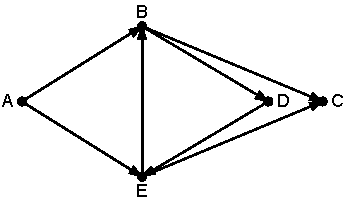
\includegraphics[width=0.50\textwidth]{Bilder/Kapitel-11/Aufrufgraph.pdf}
	\caption{Aufrufgraph}
	\label{fig:aufrufgraph}
\end{figure}

Es liegt Rekursion vor, wenn der Graph \textit{Zyklen} enthält. Eine direkte Rekursion ist ein Zyklus $(X,X)$, also eine Kante von einem Knoten zu sich selbst. Eine indirekte Rekursion entspricht einem Zyklus größerer Länge. In unserem Beispiel finden wir $(B,D), (D, E), (E,B)$ als Zyklus, der die indirekte Rekursion beschreibt.

Ein Zyklus in einem gerichteten Graphen ist visuell selbsterklärend und formal \mbox{definiert} als Kantenfolge 
$$ (X_1, X_2), (X_2, X_3), \ldots , (X_{i-1}, X_{i}), (X_{i}, X_1),$$ 
wobei für $i=1$ die Folge nur aus der Kante (Schlinge) $(X_1, X_1)$ besteht.

Um indirekte Rekursion zu erkennen, muss also der Aufrufgraph ermittelt werden, und dieser muss auf Zyklen untersucht werden. Effiziente Algorithmen, die dies leisten, lernen Sie in anderen Modulen kennen.

\vspace{1.5cm}
ENDE.

% 11.3
% Kommentierte Literatur beginnt auf neuer Seite
\clearpage
\section{Kommentierte Literatur}
\label{sec:Kap-11.3}

\sttpKommLitItem{Ludewig/Lichter}{2023}{Software Engineering}{lud23}{}{}
{In Kapitel~18 "`Programmtest"' werden generelle Konzepte des Testens im Software\-entwicklungs\-prozess angesprochen. Dazu zählen das Einordnen von Tests in den Gesamtlebenszyklus, grundlegende Teststrategien sowie ein Überblick über verschiedene Teststufen. Die Darstellung ist eher breit gefasst und soll ein allgemeines Verständnis vermitteln.}

\sttpKommLitItem{Spillner/Linz}{2019}{Basiswissen Softwaretest}{spi19}{}{}
{Eine ausführliche Betrachtung des Programmtests. Dieses Buch ist als etablierter Standard für die Vorbereitung auf den ISTQB-Certified-Tester bekannt. Ent\-sprechend bietet es einen tieferen Einblick in methodische und praktische Aspekte des Software-Testens. Es finden sich ausführliche Darstellungen von Testfallentwurfsverfahren, dynamischen und statischen Testtechniken, Testdokumentation, Test\-organisation, Rollen und Verantwortlichkeiten im Testprozess sowie ein stärkerer Fokus auf Normen, Standards und das professionelle Testmanagement.}

\sttpKommLitItem{Hoare}{1969}{An Axiomatic Basis for Computer Programming}{hoa69}{}{}
{Hoare legt in seinem grundlegenden Artikel den theoretischen Grundstein für formale Korrektheitsbeweise von Programmen. Historische Grundlagenliteratur.}

\sttpKommLitItem{Huth/Ryan}{2004}{Logic in Computer Science}{hut04}{}{}
{Kapitel~4 "`Program verification"' bietet einen vertieften Einblick in die formale Verifikation von Programmen. Behandelte Themen umfassen unter anderem Hoare-Tripel, partielle und totale Korrektheit sowie grundlegende Beweisregeln und Verifikations\-strategien.}